\documentclass{beamer}

\usepackage{graphicx}                           % per le immagini
\usepackage{float}                              % per posizionare le immagini esattamente come appaiono nel testo

\usepackage[backend=bibtex,style=ieee]{biblatex}
\bibliography{bibliografia}

% Use Unipd as theme, with options:
% - pageofpages: define the separation symbol of the footer page of pages (e.g.: of, di, /, default: of)
% - logo: position another logo near the Unipd logo in the title page (e.g. department logo), passing the second logo path as option 
\usetheme[pageofpages=of,logo=dei_logo.png]{Unipd}

\title{Compressione di immagini tramite autoencoder}
\subtitle{stato dell’arte e sviluppi futuri}
\author[Filippo Stella, Marco Cagnazzo]{F.~Stella \and M.~Cagnazzo}

\date{16 Novembre 2023}

% The next block of commands puts the table of contents at the beginning of each section and highlights the current section
% \AtBeginSection[]
% {
%   \begin{frame}
%     \frametitle{Table of Contents}
%     \tableofcontents[currentsection]
%   \end{frame}
% }

\begin{document}

% Make the title page
\frame{\titlepage}

% Insert the general toc
\begin{frame}{Indice}
    \tableofcontents    
\end{frame}

\section{Compressione}

    \begin{frame}{Compressione}
        \begin{figure}[t!]
            \centering
            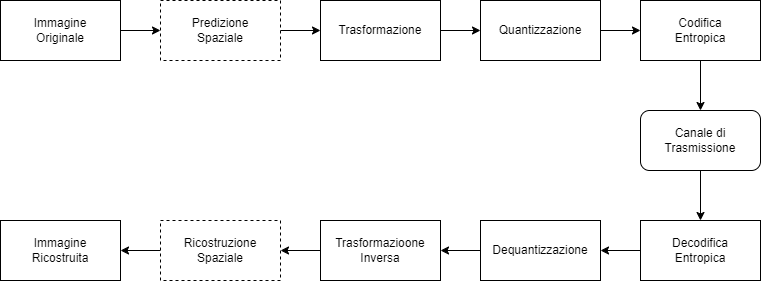
\includegraphics[width=0.8\textwidth]{Immagini/LossyCompressorDiagram.png}
            \caption{Blocchi funzionali principali di un framework lossy \cite{sadeeq2021image}, con l’aggiunta di un quarto blocco per i metodi recenti}
            \label{fig:LossyCompressorDiagram}
        \end{figure}
    \end{frame}
\section{Metodi tradizionali}

    \begin{frame}{Metodi Tradizionali}
        I metodi di codifica tradizionale analizzati in questo studio sono i seguenti
        \begin{itemize}
            \item JPEG\footnotemark[1]
            \item JPEG 2000\footnotemark[2]
            \item BPG\footnotemark[3]
            \item VVC\footnotemark[4]
        \end{itemize}
        \footnotetext[1]{\fullcite{125072}}
        \footnotetext[2]{\fullcite{952804}}
        \footnotetext[3]{\fullcite{BPGImageformat}}
        \footnotetext[4]{\fullcite{9503377}}
    \end{frame}
        
\section{Metodi con reti neurali}

    \begin{frame}{Autoencoder}
        \begin{figure}[t!]
            \centering
            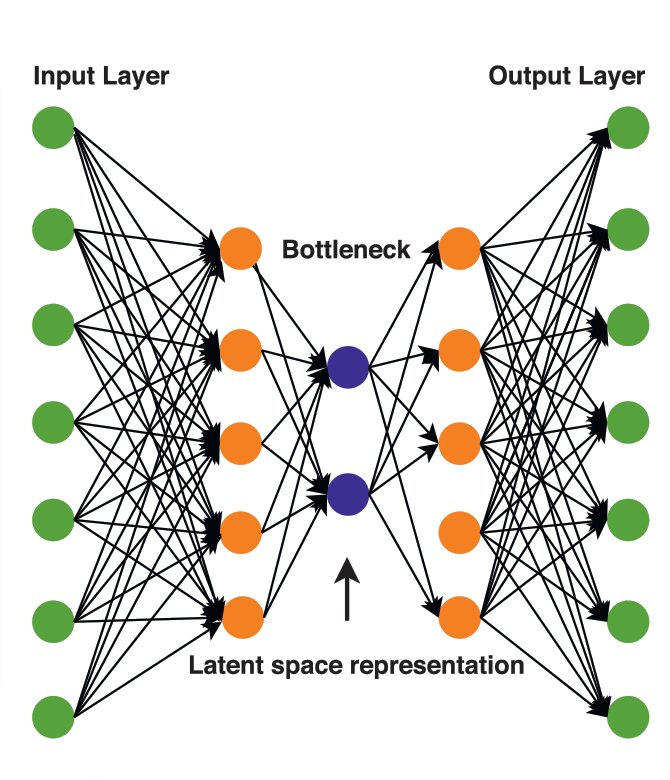
\includegraphics[width=0.5\textheight]{Immagini/Autoencoder_scheme.png}
            \caption{Schema generico di un autoencoder, immagine presa dal documento \textit{Deep architectures for image compression: A critical review}\footnotemark[1]}
            \label{fig:schemeAutoencoder}
        \end{figure}
        \footnotetext[1]{\fullcite{mishra2022deep}}
    \end{frame}

    \begin{frame}{Metodi con reti neurali}
        I metodi di codifica con reti neurali analizzati in questo studio sono i seguenti
        \begin{itemize}
            \item Variational compression with a scale hyperprior, Ballé et al\footnotemark[1].
            \item Discretized gaussian mixture likelihoods, Cheng et al\footnotemark[2].
            \item Neural data-dependent transform, Wang et al\footnotemark[3]. 
        \end{itemize}
        \footnotetext[1]{\fullcite{minnen2018joint}}
        \footnotetext[2]{\fullcite{cheng2020learned}}
        \footnotetext[3]{\fullcite{wang2022neural}}
    \end{frame}

    \begin{frame}{Ballé et al\footnotemark[1]. 2018}
        \begin{figure}[!h]
            \centering
            \includegraphics[width=0.7\textheight]{Immagini/Ballé2018_Rete.png}
            \caption{Diagramma rete Ballé 2018 et al., immagine presa dal documento \textit{Joint autoregressive and hierarchical priors for learned image compression}\footnotemark[1]}
            \label{fig:balle2018Network}
        \end{figure}
        \footnotetext[1]{\fullcite{minnen2018joint}}
    \end{frame}

    \begin{frame}{Cheng et al\footnotemark[1]. 2020}
        \begin{figure}[!h]
            \centering
            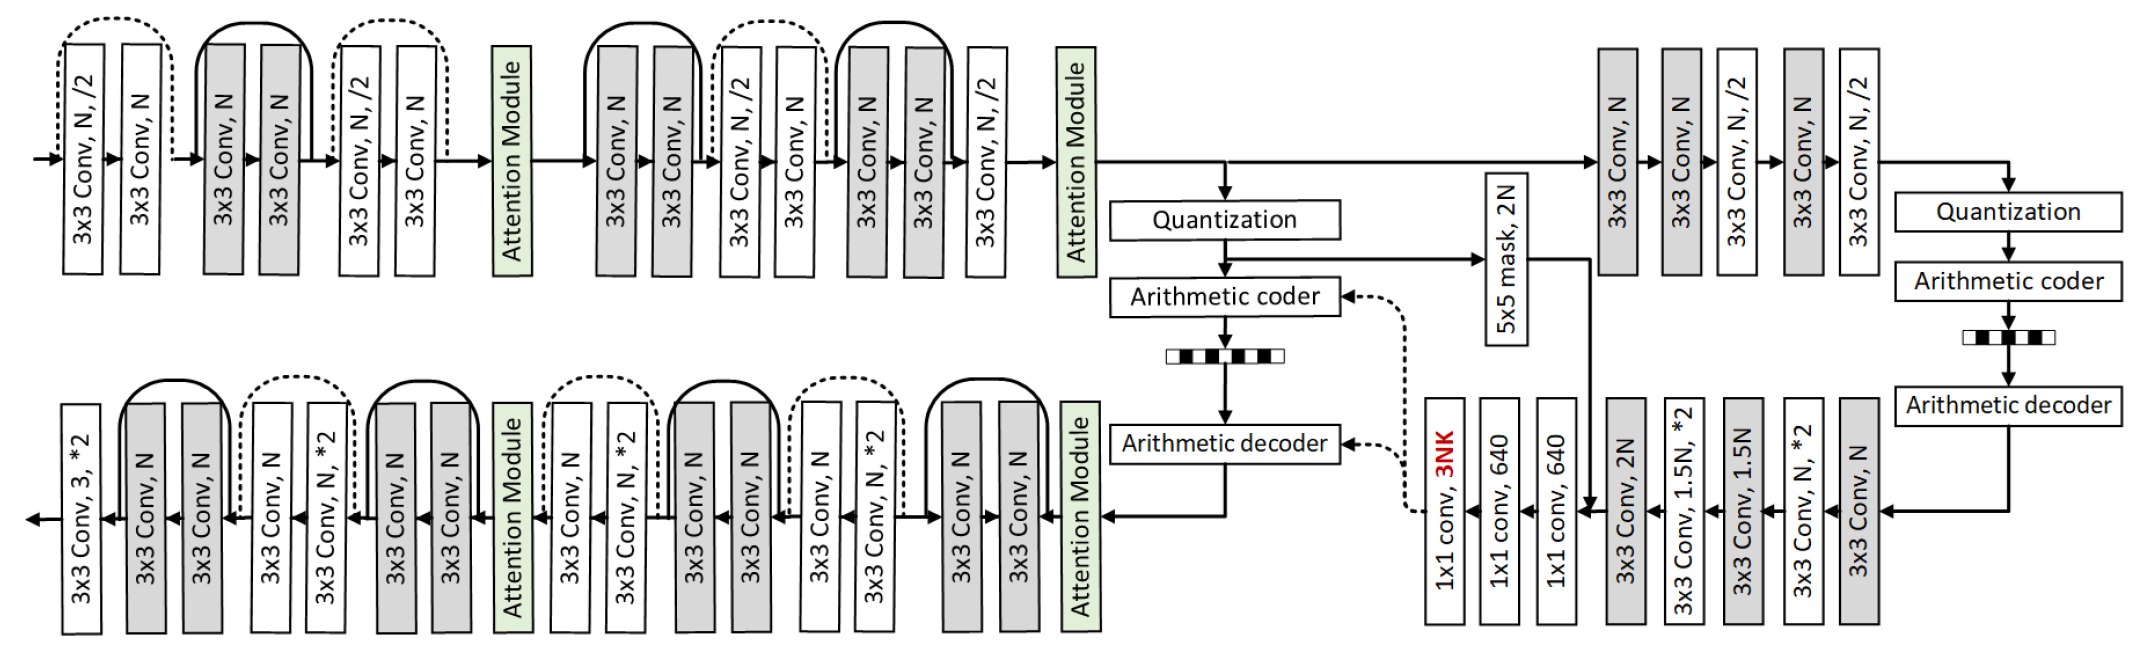
\includegraphics[width=1\textwidth]{Immagini/Cheng2020_Rete.png}
            \caption{Diagramma rete Cheng 2020 et al., immagine presa dal documento \textit{Learned image compression with discretized gaussian mixture likelihoods and attention modules}\footnotemark[1]}
            \label{fig:cheng2020Network}
        \end{figure}
        \footnotetext[1]{\fullcite{cheng2020learned}}
    \end{frame}

    \begin{frame}{Wang et al\footnotemark[1]. 2022}
        \begin{figure}[!h]
            \centering
            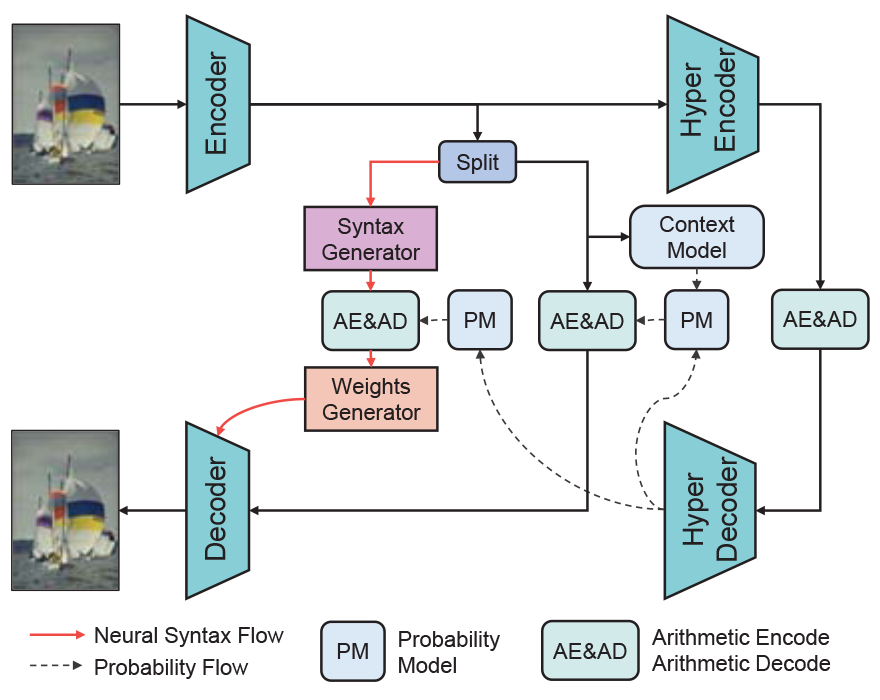
\includegraphics[width=0.6\textheight]{Immagini/Wang2022_Rete.png}
            \caption{Diagramma rete Wang 2022 et al., immagine presa dal documento \textit{Neural data-dependent transform for learned image compression}\footnotemark[1]}
            \label{fig:Wang2022Network}
        \end{figure}
        \footnotetext[1]{\fullcite{wang2022neural}}
    \end{frame}
    
\section{Risultati Sperimentali}

    \begin{frame}{Esempi di Compressione}
        Esempi di compressione di un immagine a 24bpp del dataset Kodak\footnotemark[1] con le tecniche presentate\\
        \begin{figure}[!ht]
            \begin{minipage}[]{0.13\linewidth}
                \centering
                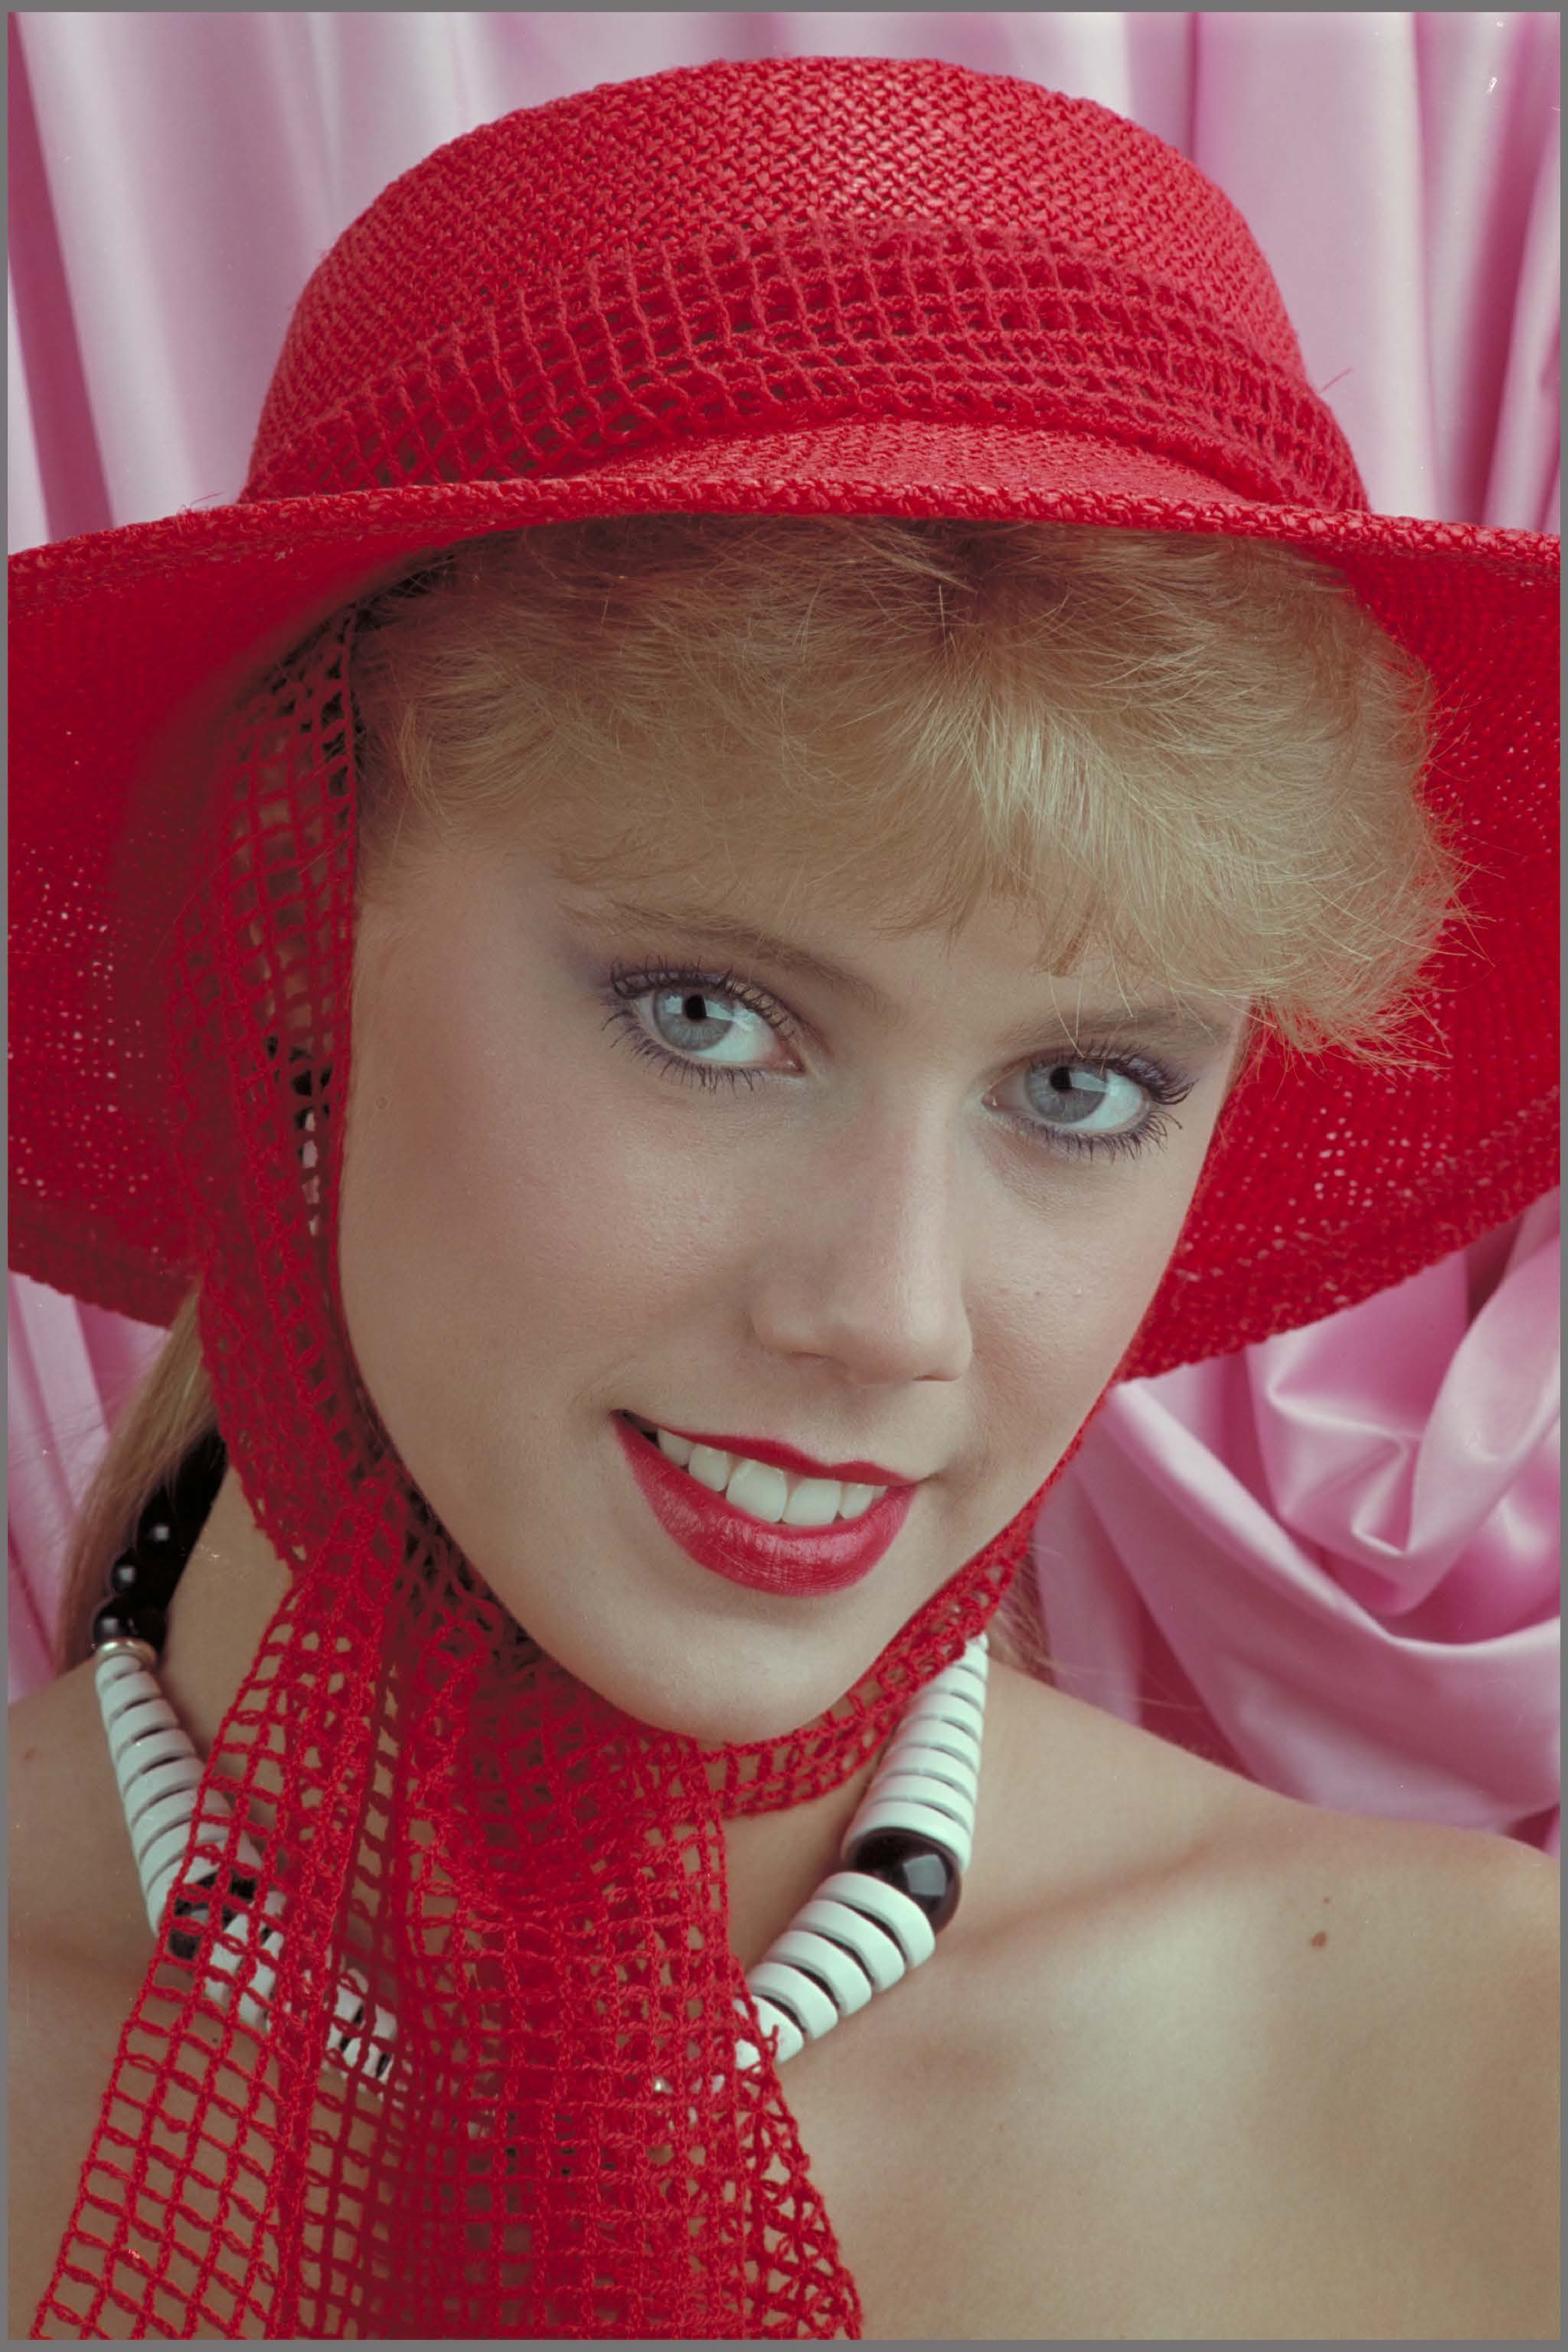
\includegraphics[width=\textwidth]{Immagini/IMAGES/PNG_IMG0004.pdf}
                \caption{Lossless 11.117bpp}
                \label{fig:Lossless}
            \end{minipage}
            \begin{minipage}[]{0.13\linewidth}
                \centering
                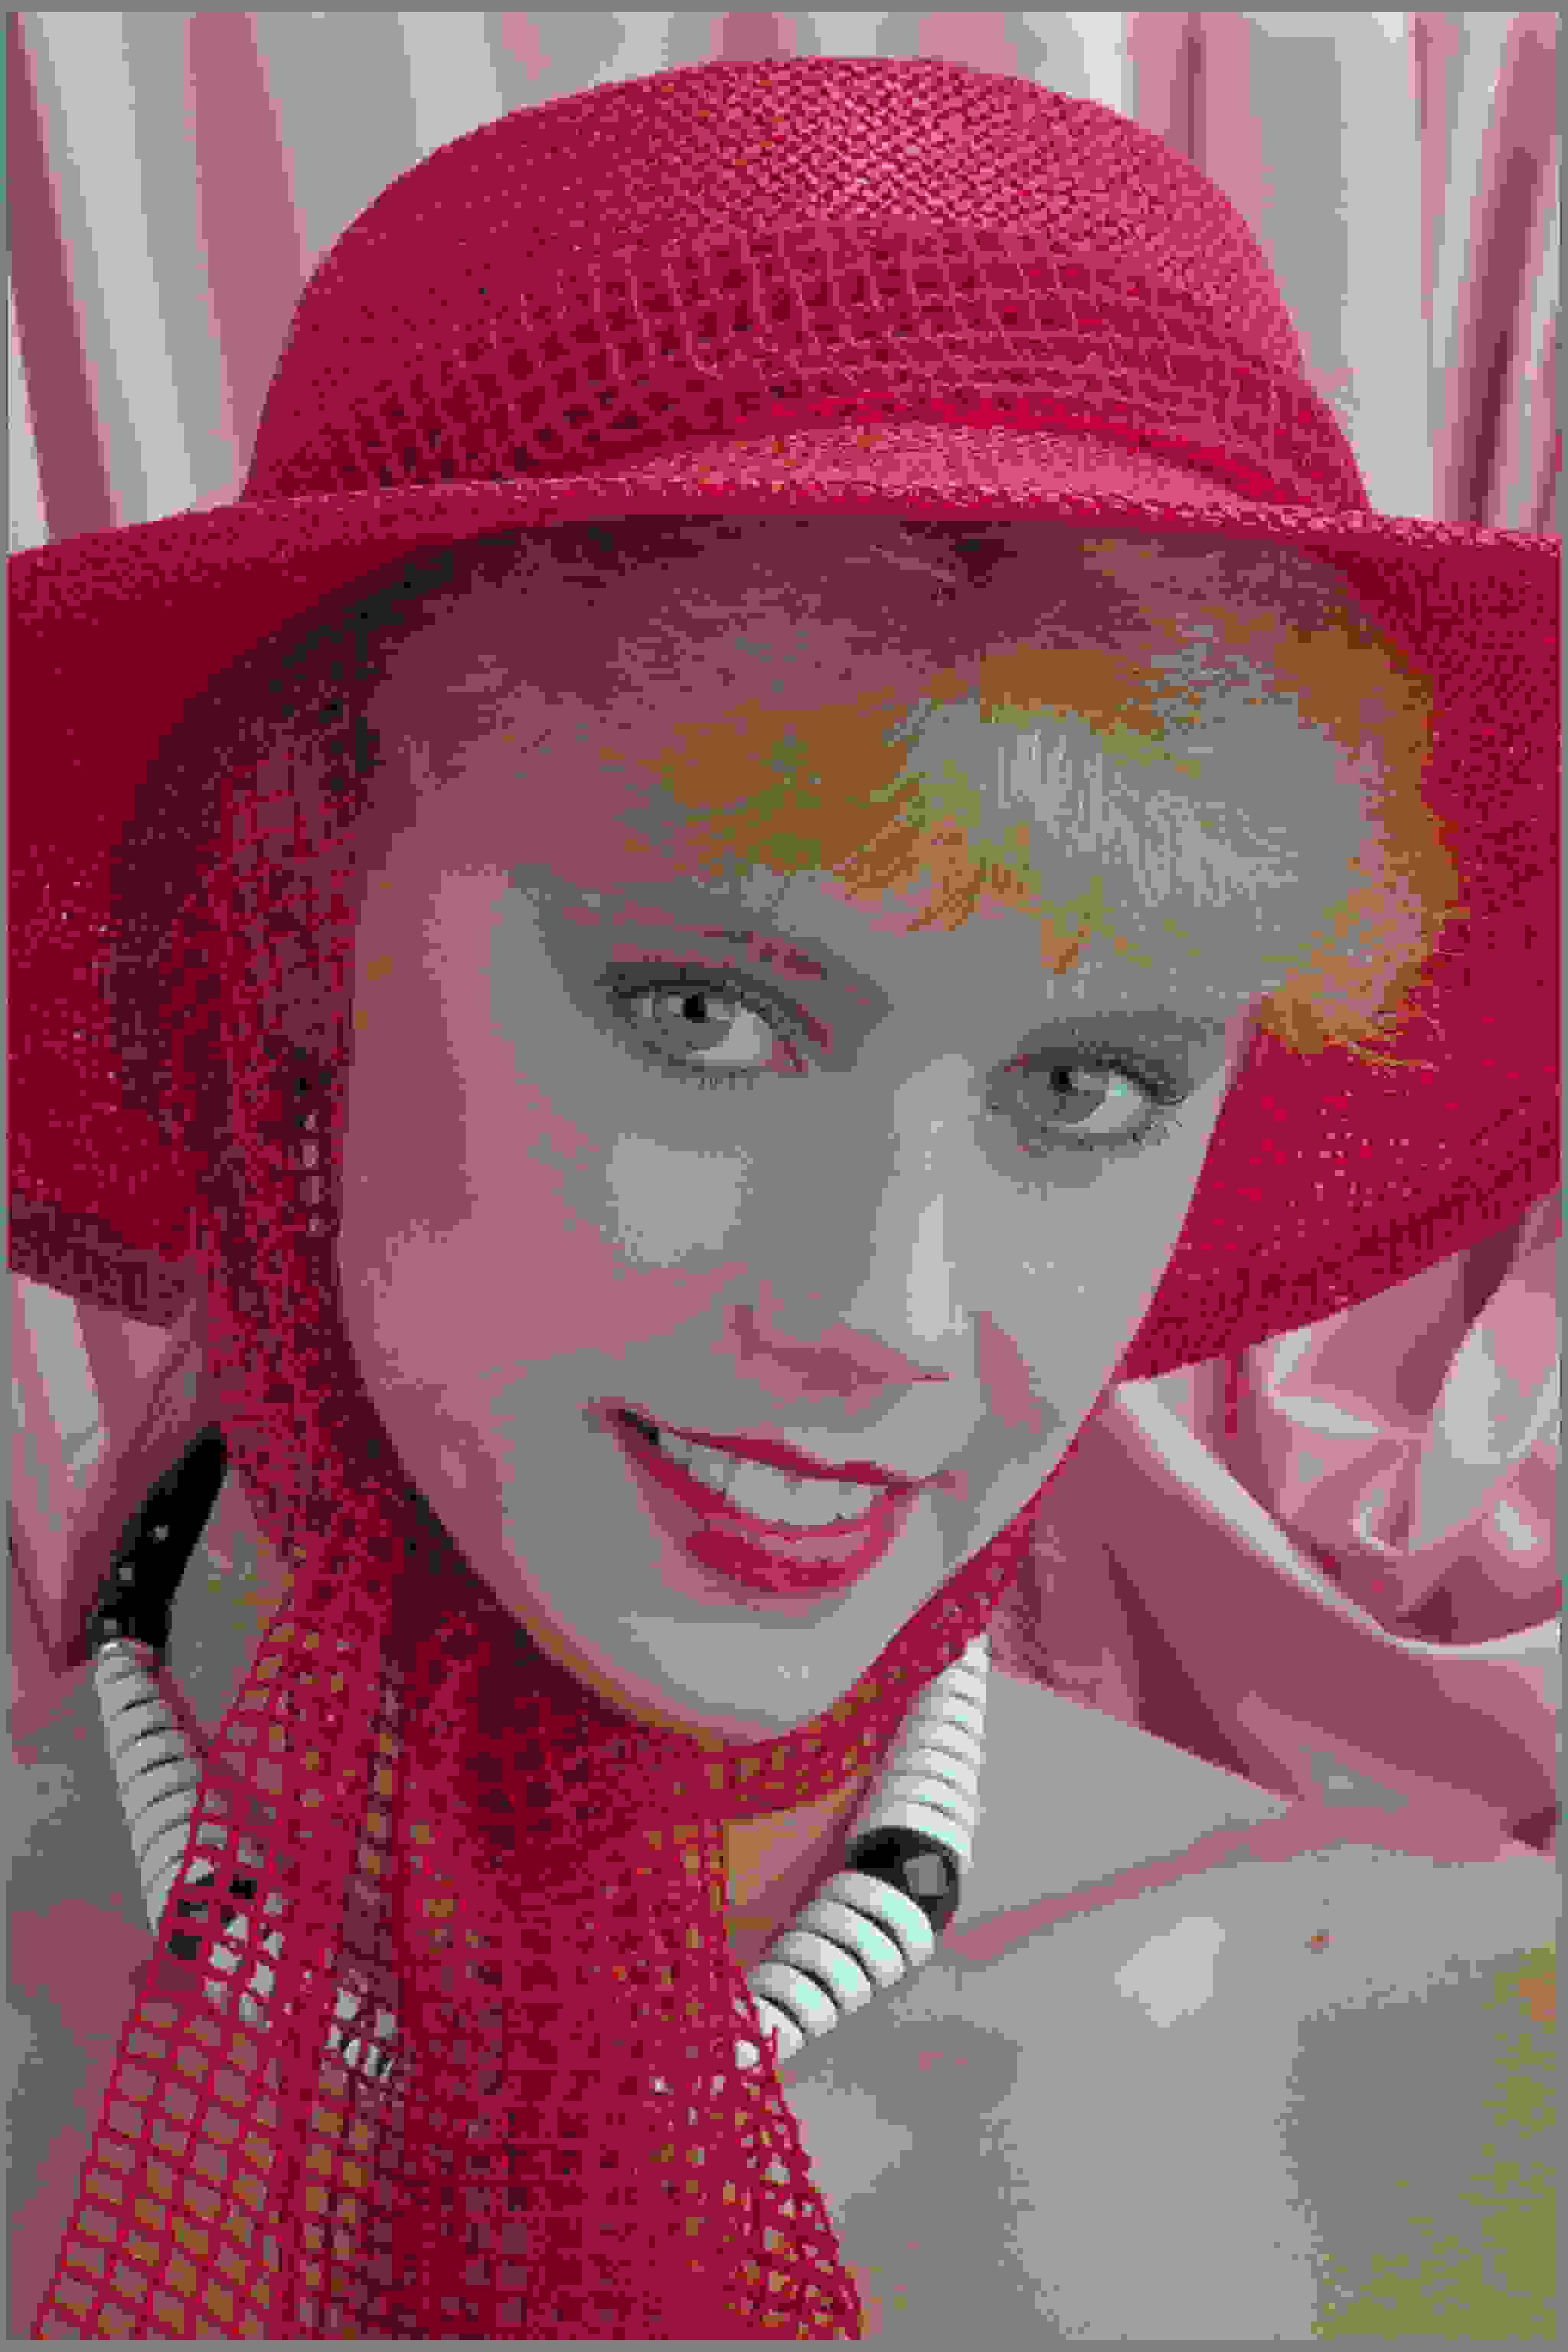
\includegraphics[width=\textwidth]{Immagini/IMAGES/JPEG_1_IMG0004.pdf}
                \caption{JPEG 0.167bpp}
                \label{fig:ExampleJPEG}
            \end{minipage}
            \begin{minipage}[]{0.13\linewidth}
                \centering
                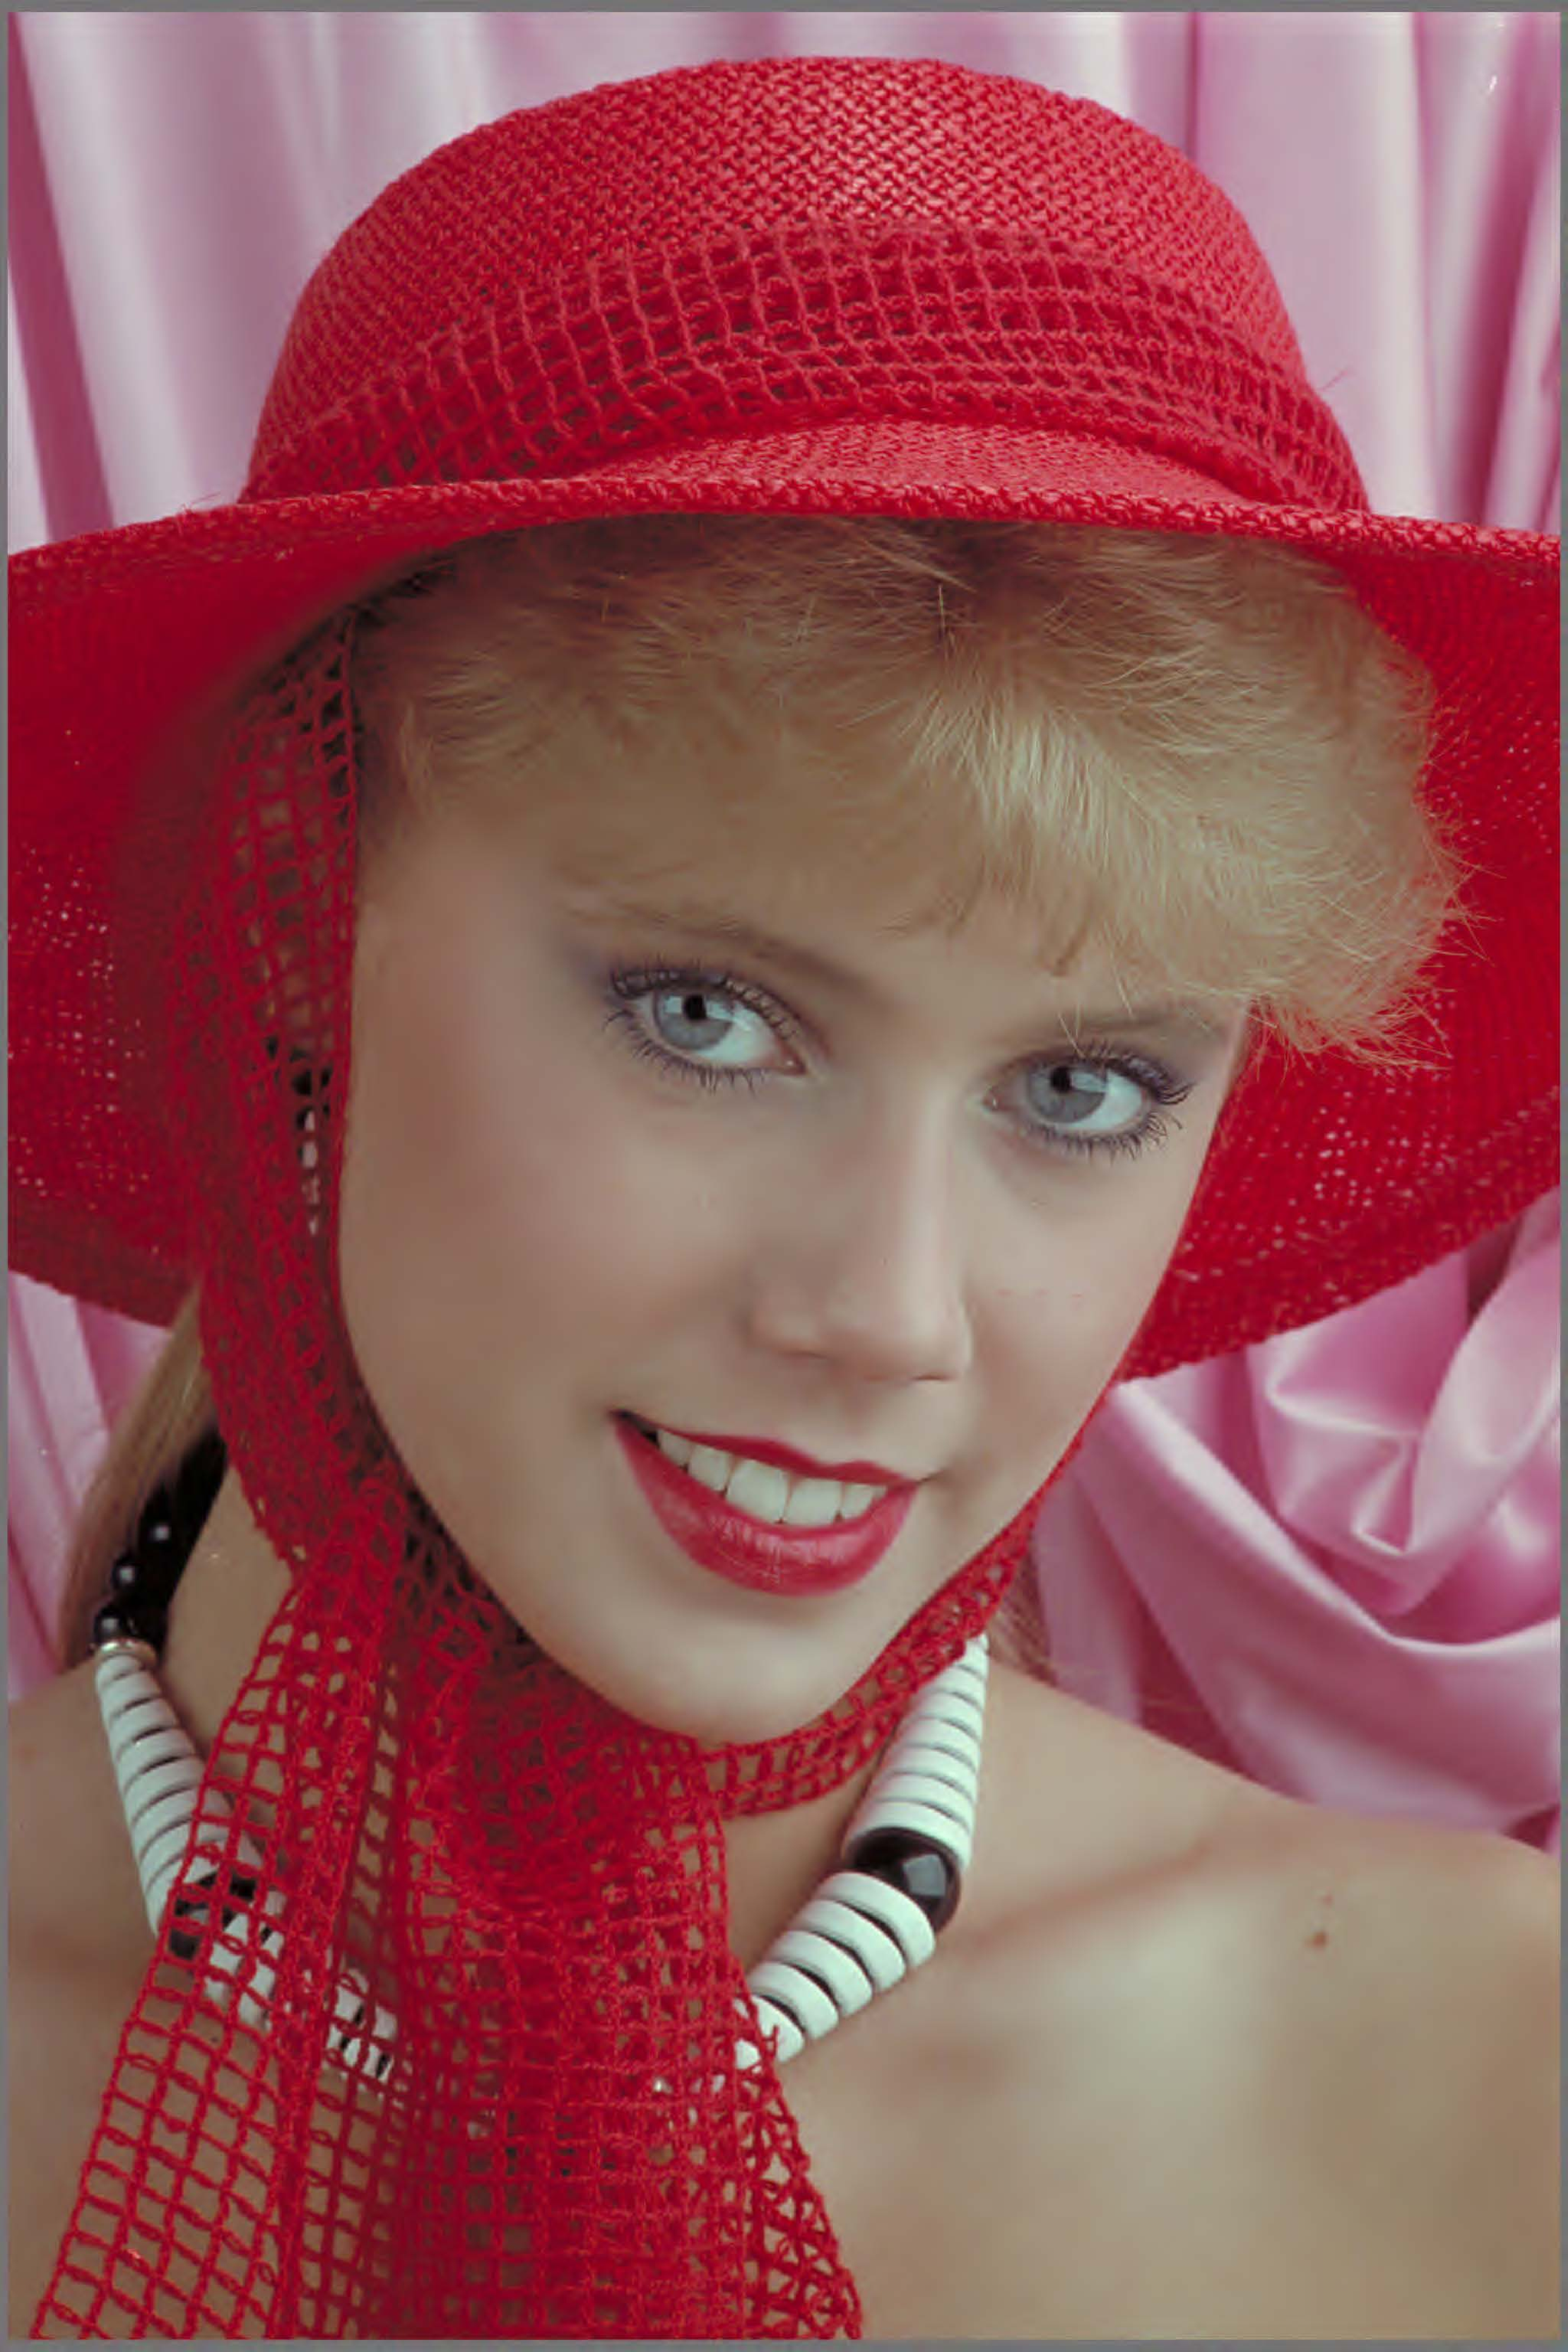
\includegraphics[width=\textwidth]{Immagini/IMAGES/JPEG2000_1_IMG0004.pdf}
                \caption{JPEG2000 0.137bpp}
                \label{fig:ExampleJPEG2000}
            \end{minipage}
            \begin{minipage}[]{0.13\linewidth}
                \centering
                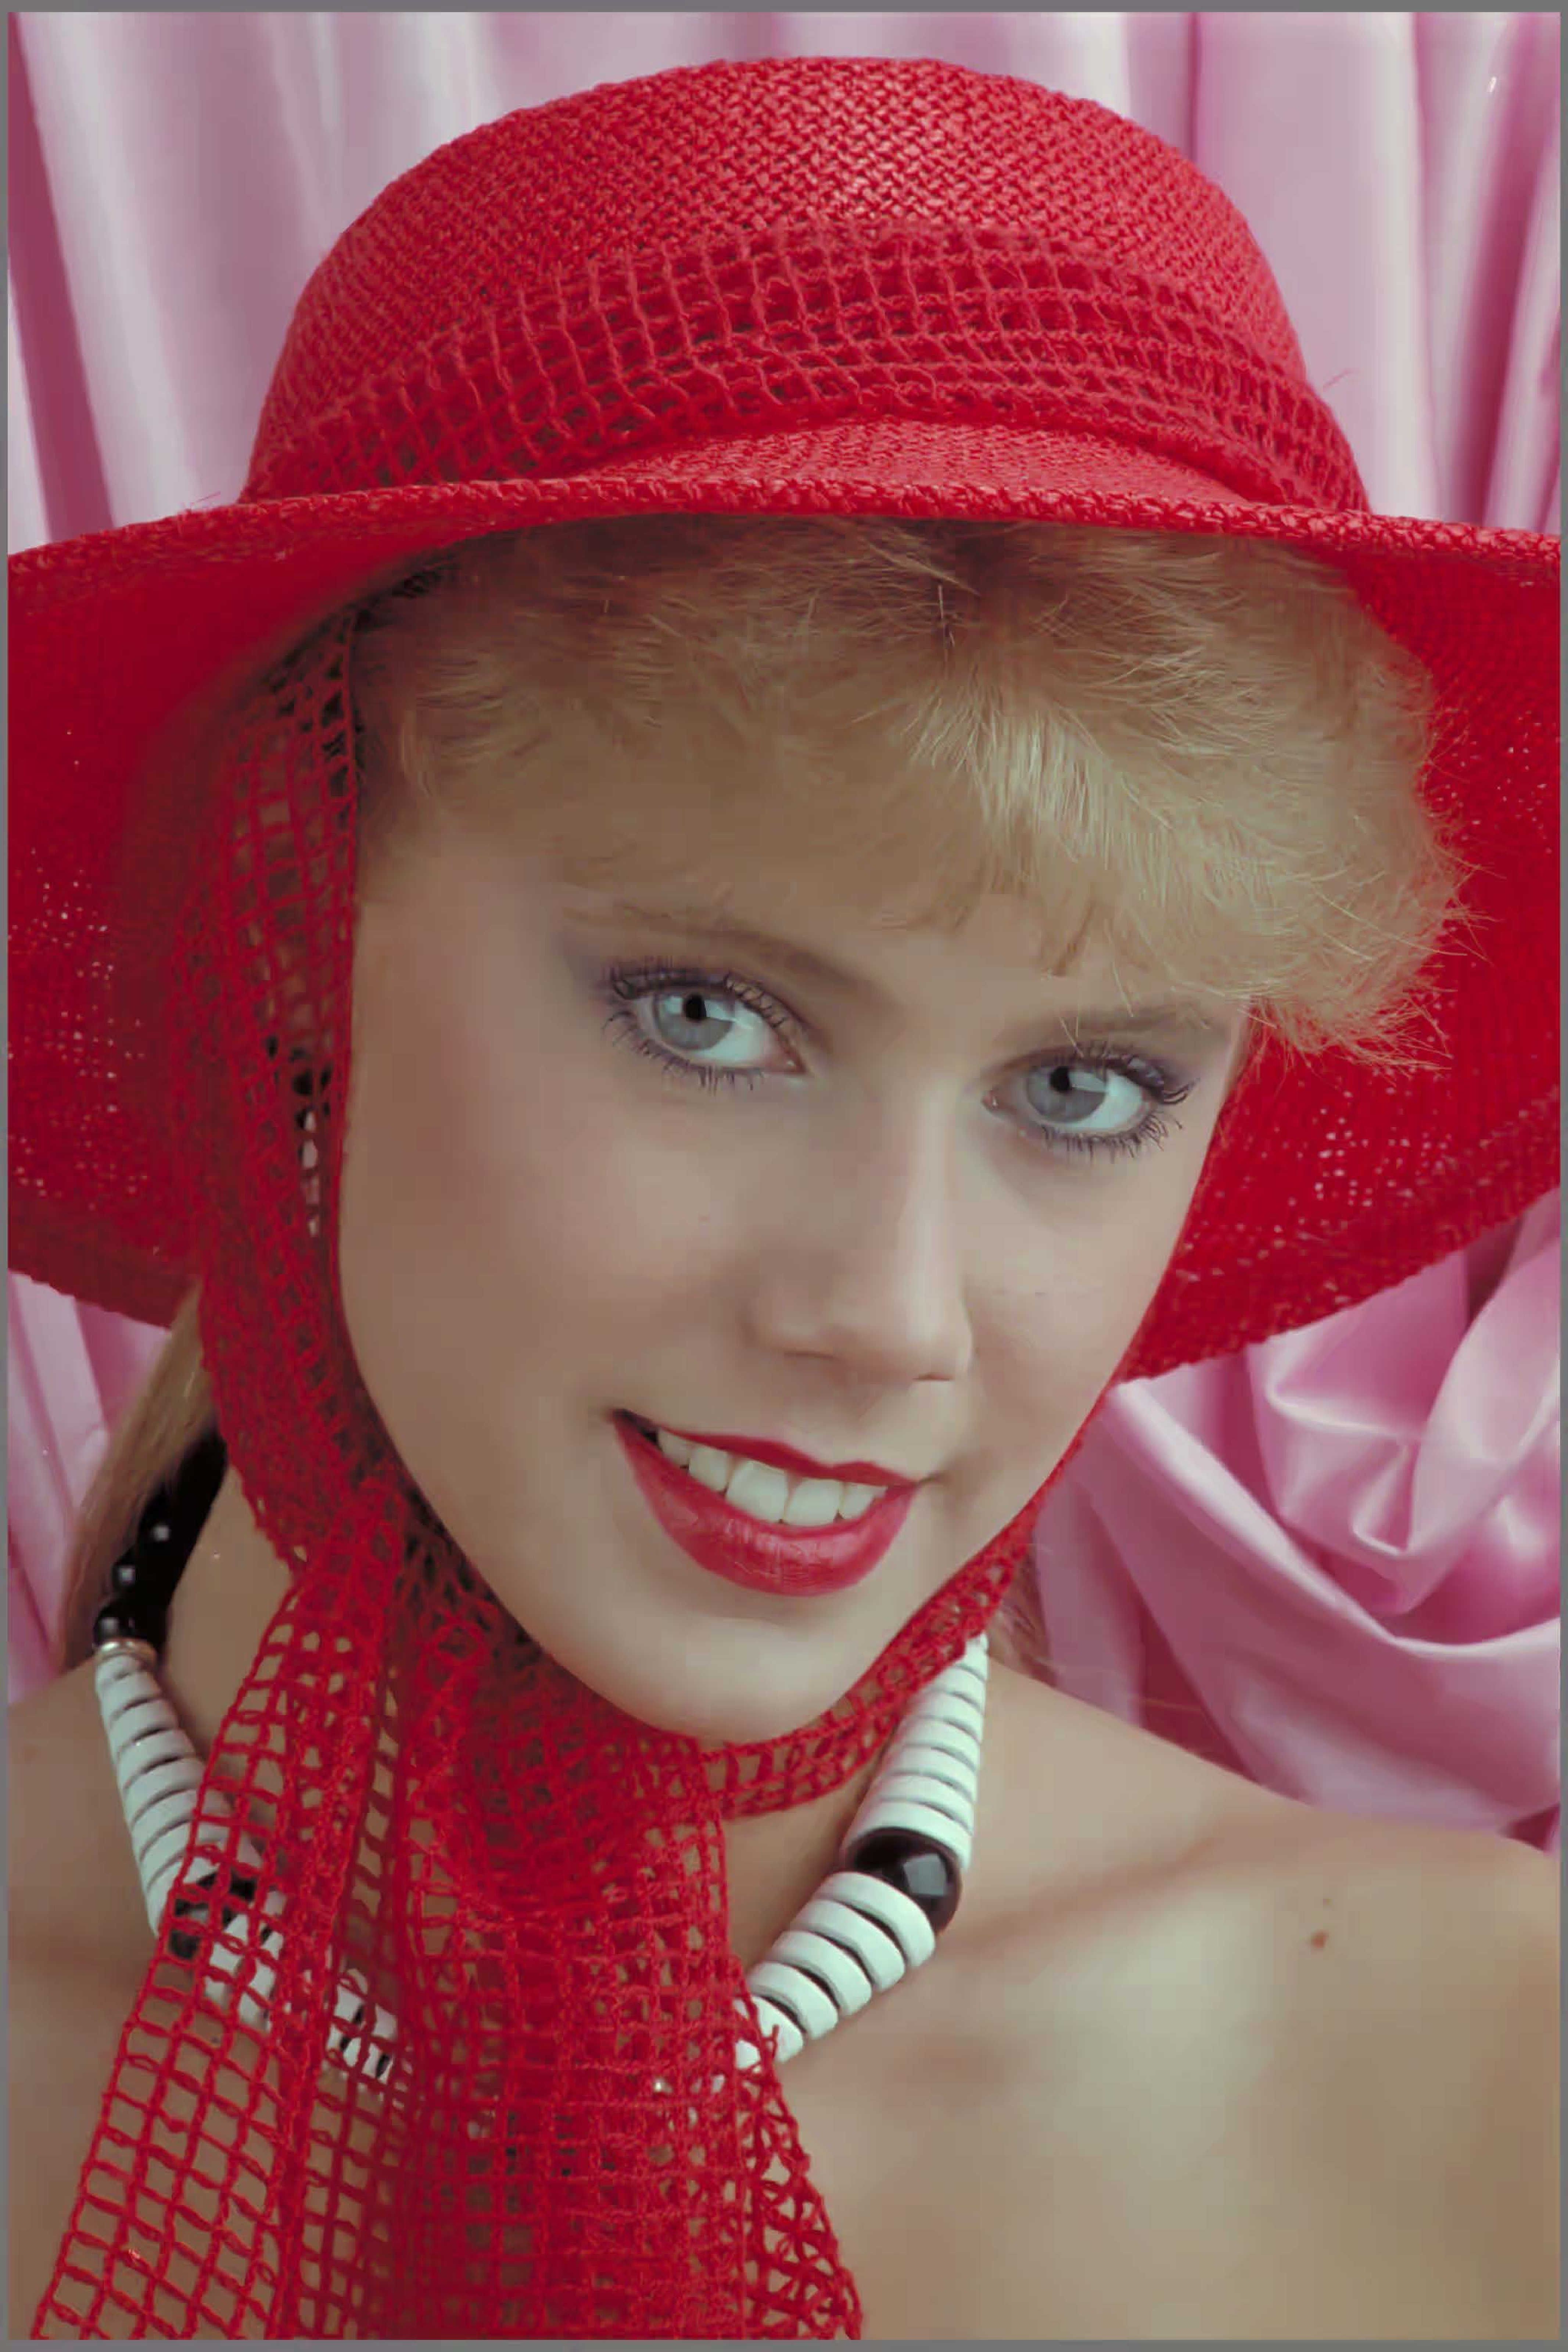
\includegraphics[width=\textwidth]{Immagini/IMAGES/BPG_2_IMG0004.pdf}
                \caption{BPG 0.103bpp}
                \label{fig:ExampleBPG}
            \end{minipage}
            \begin{minipage}[]{0.13\linewidth}
                \centering
                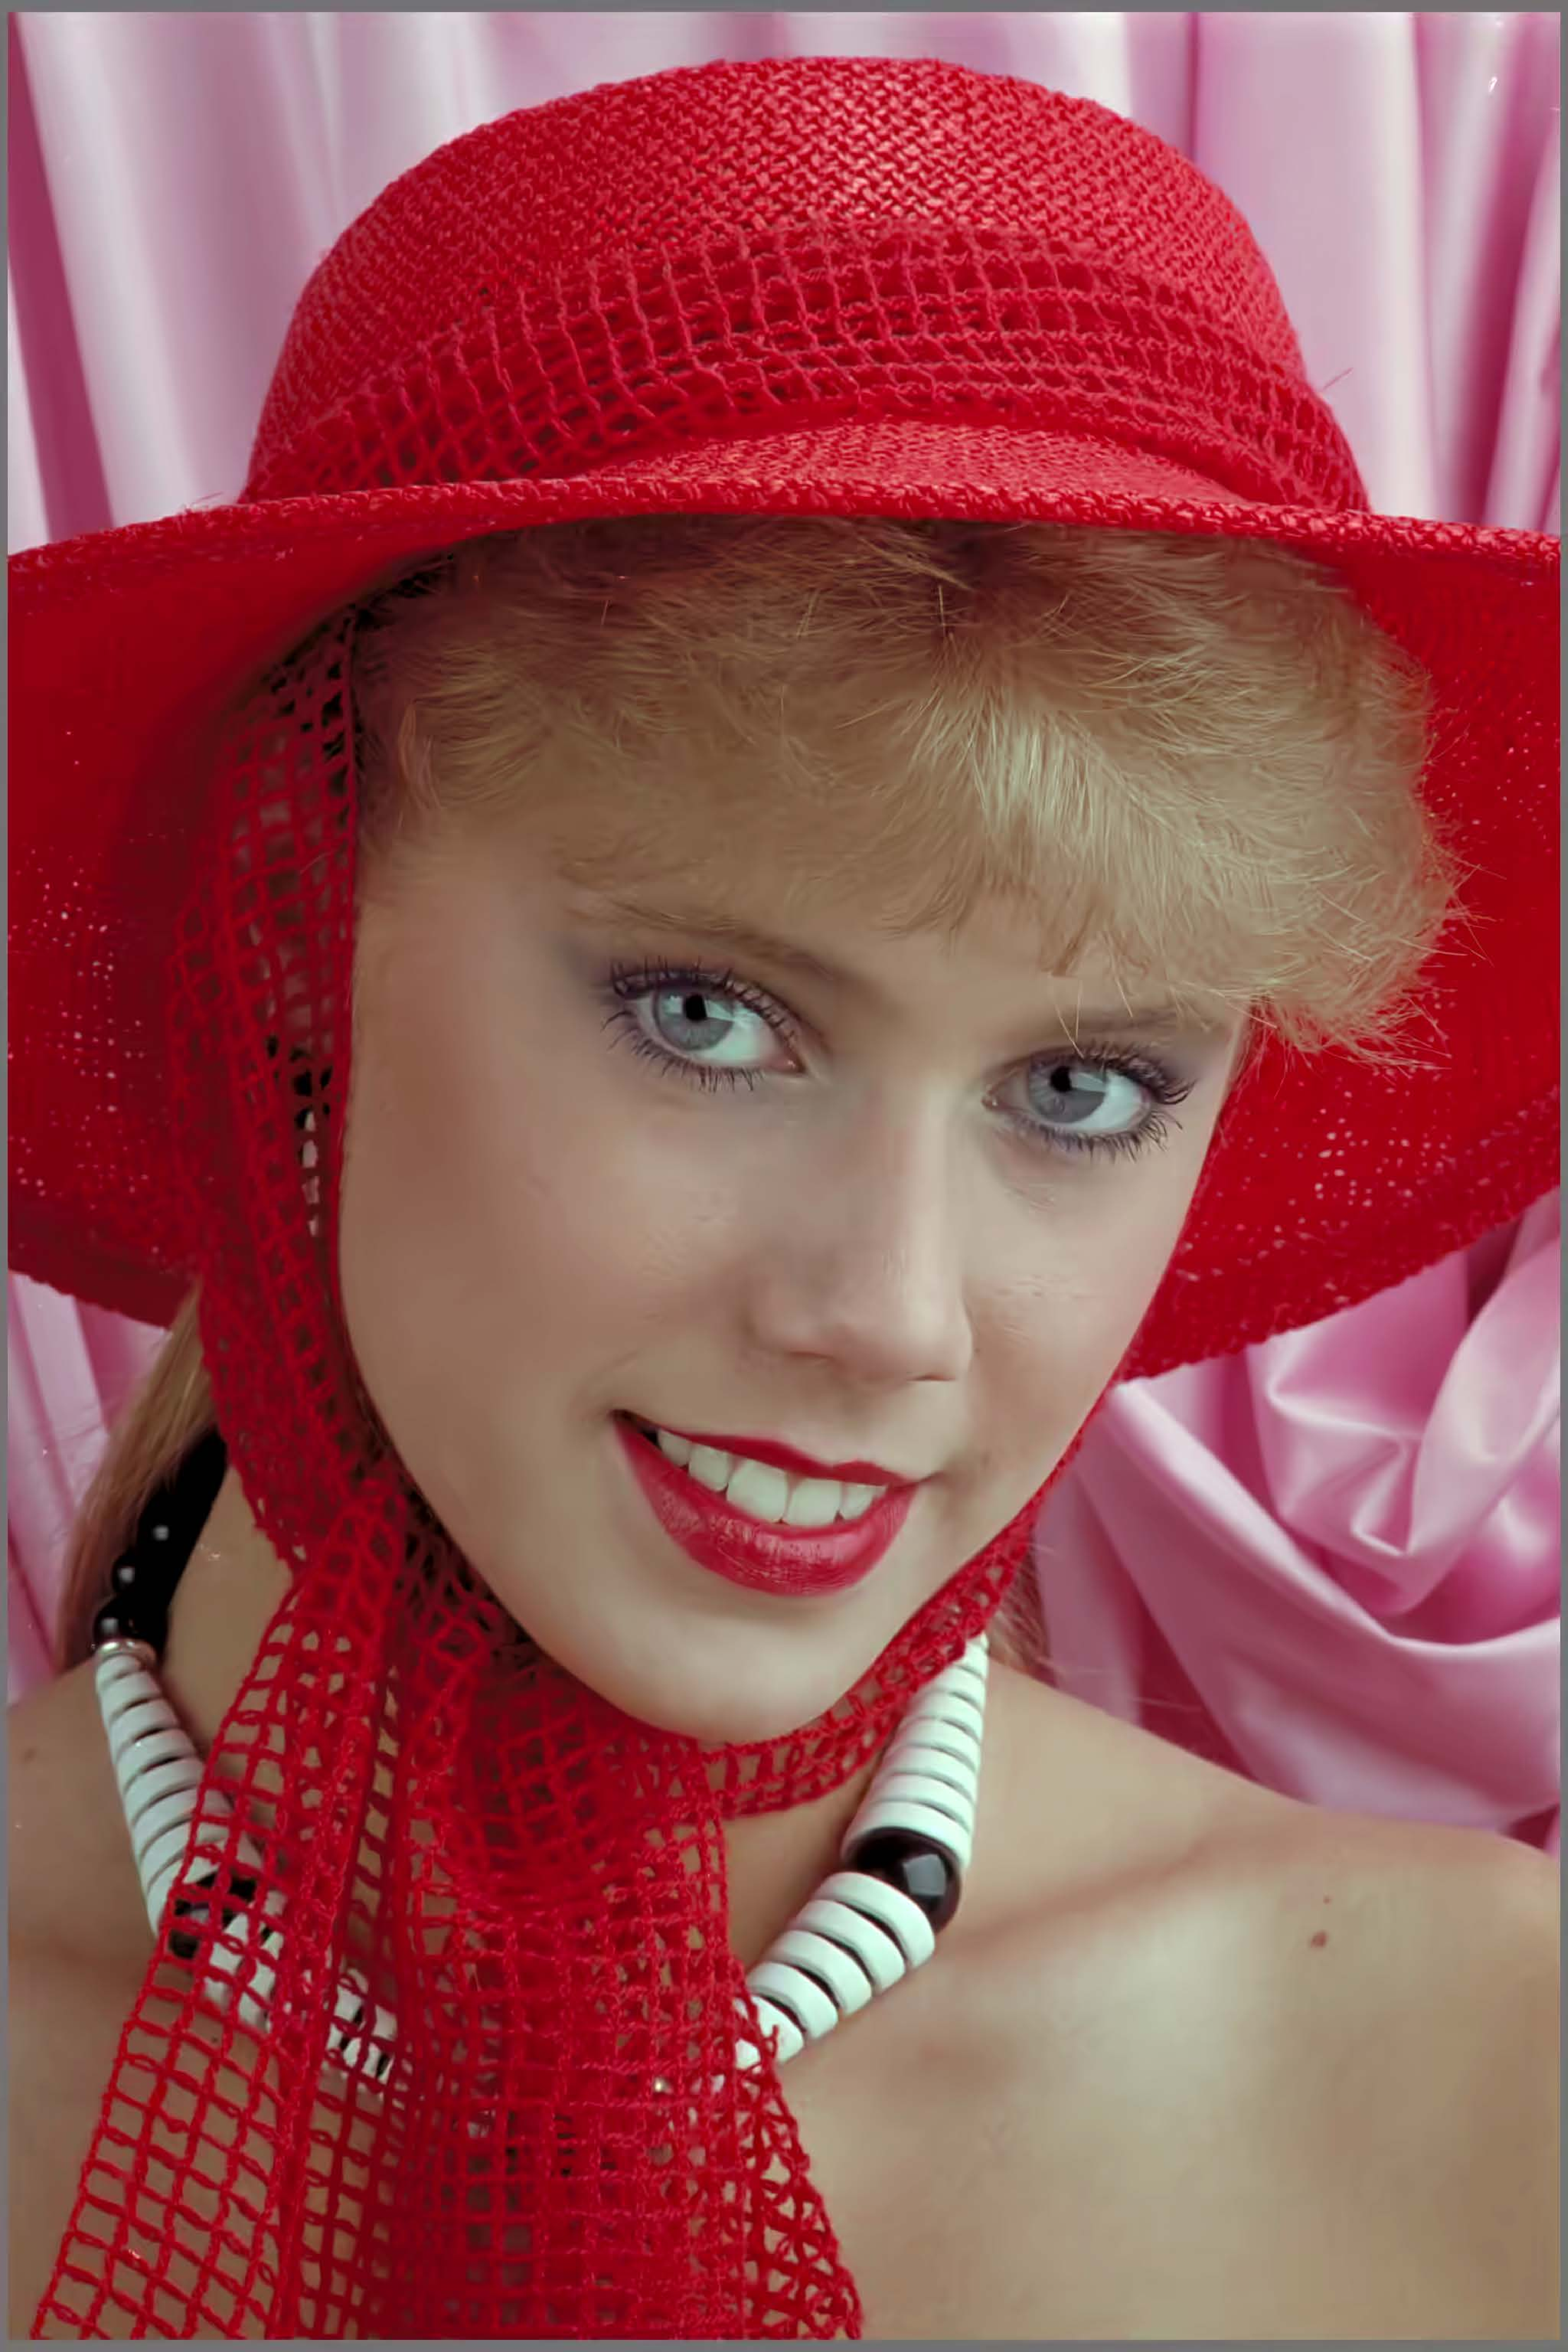
\includegraphics[width=\textwidth]{Immagini/IMAGES/VVC_1_IMG0004.pdf}
                \caption{VVC 0.061bpp}
                \label{fig:ExampleVVC}
            \end{minipage}
            \begin{minipage}[]{0.13\linewidth}
                \centering
                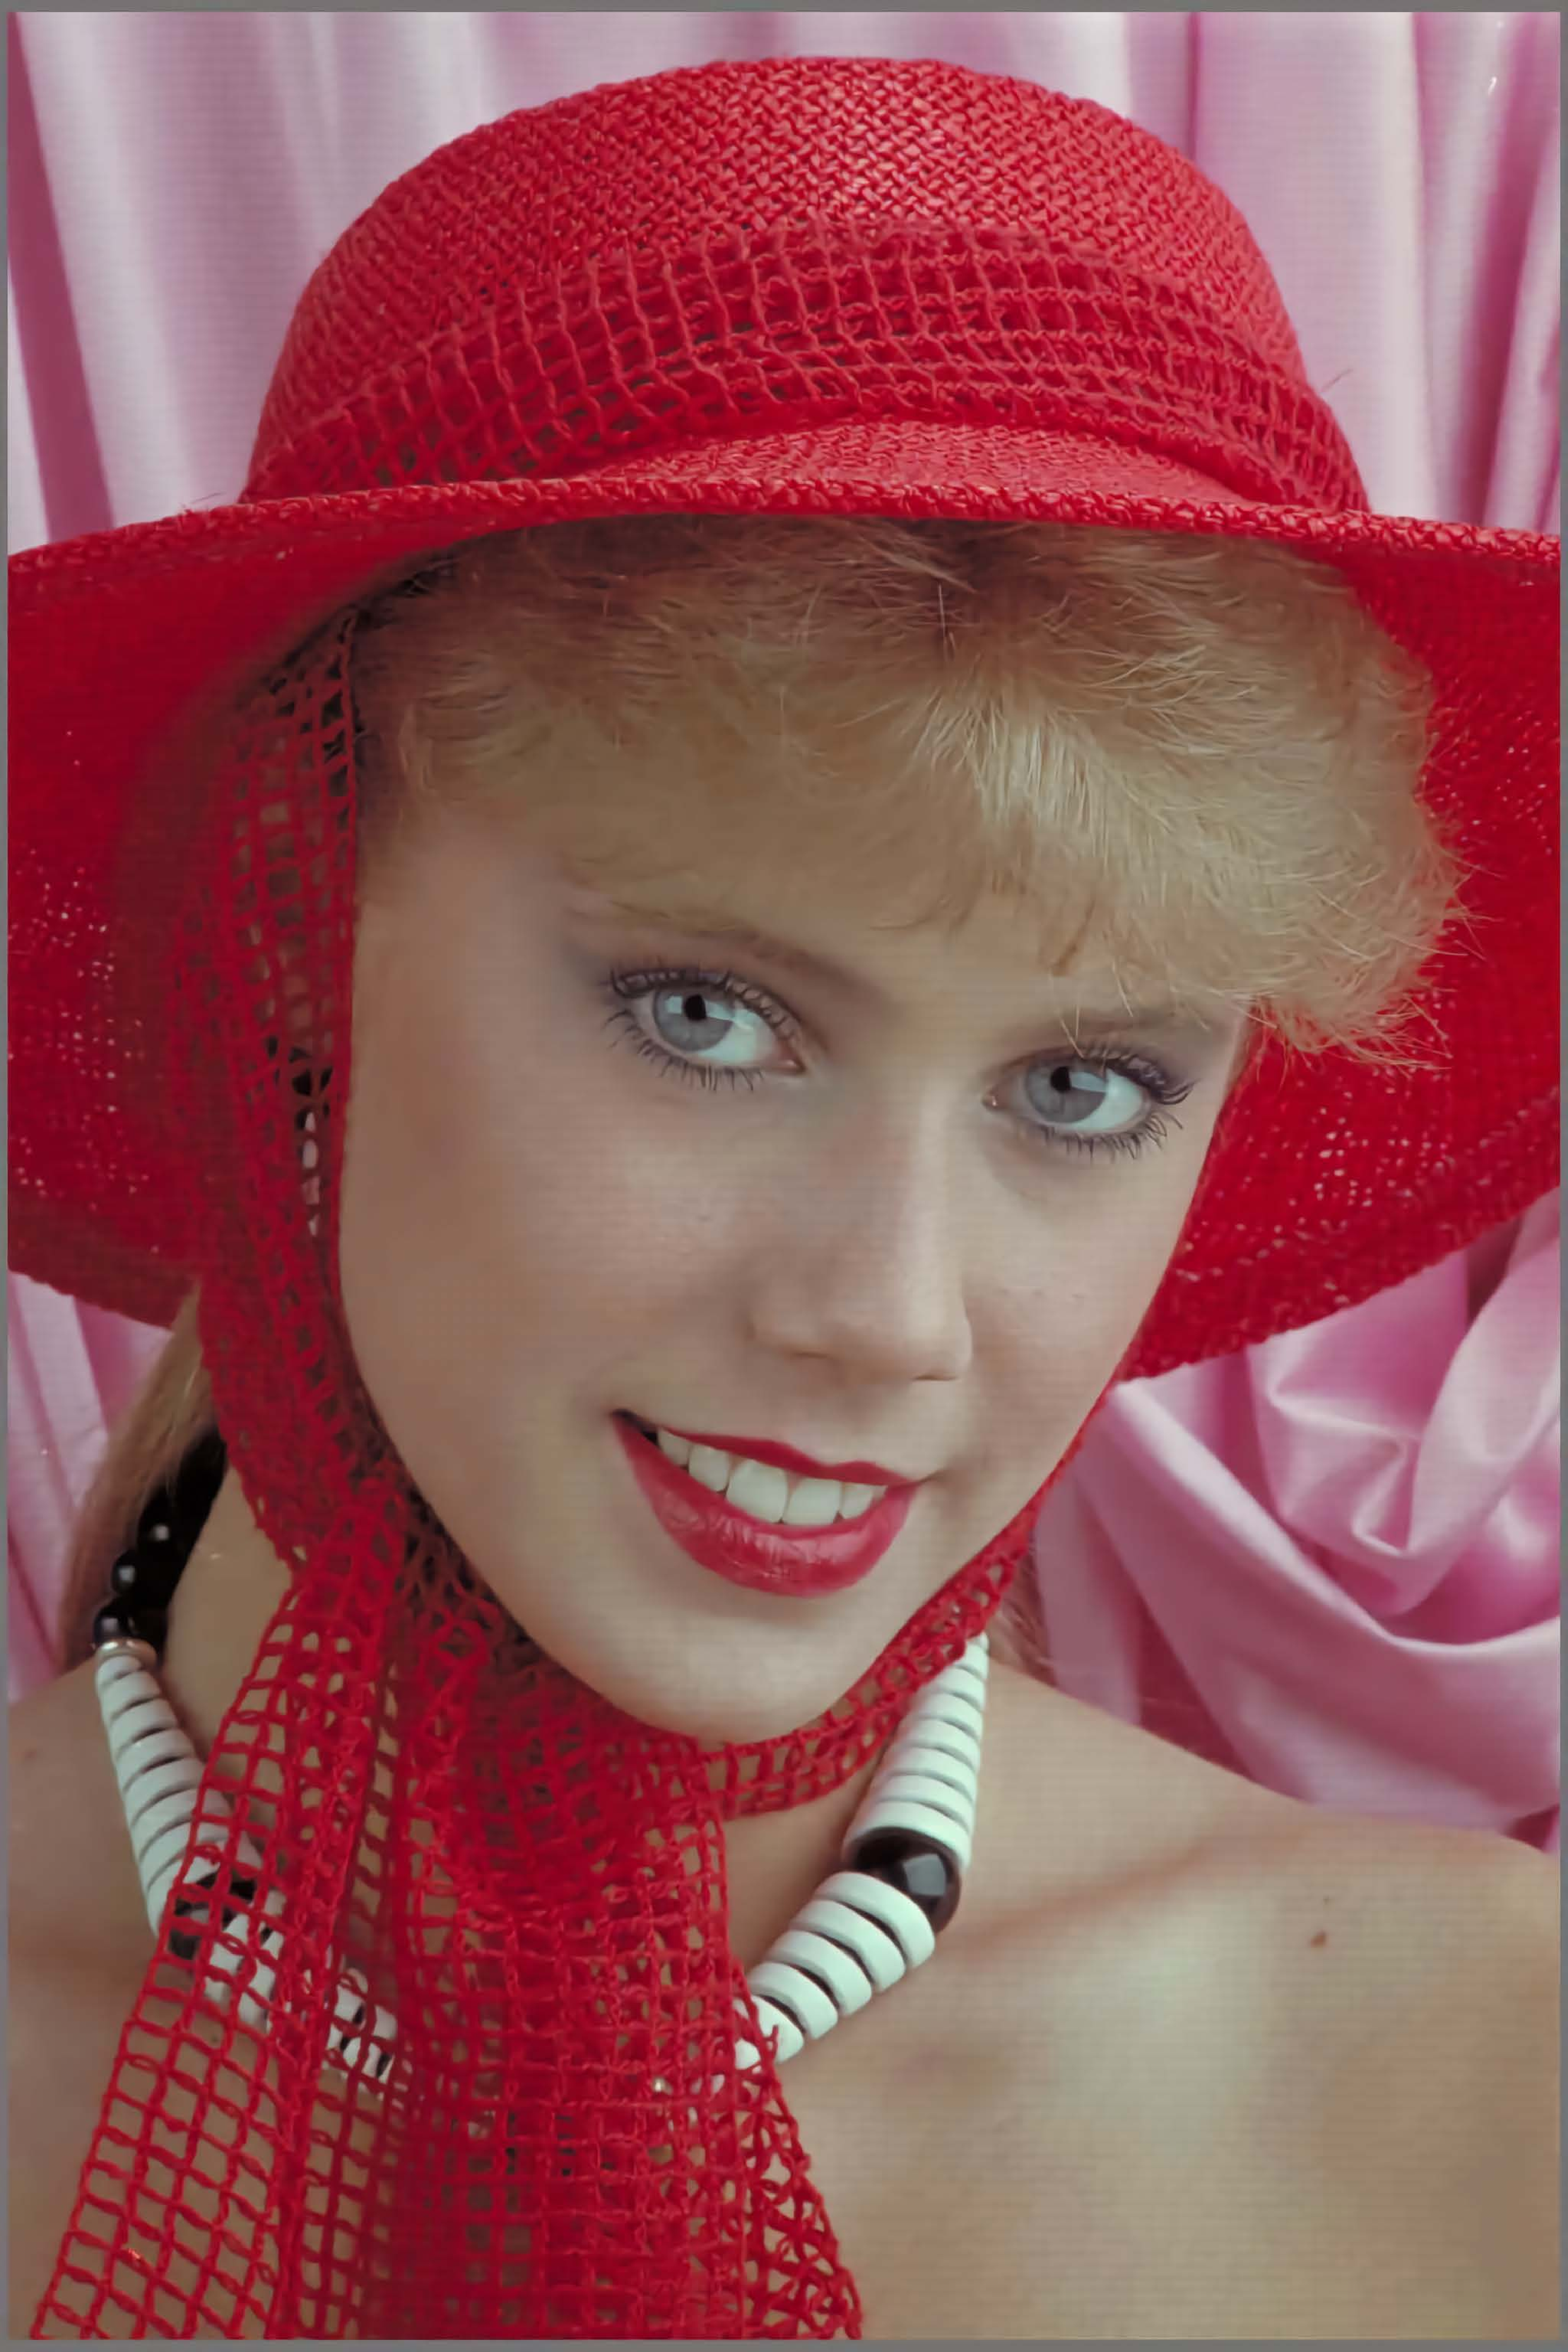
\includegraphics[width=\textwidth]{Immagini/IMAGES/mbt2018_2_IMG0004.pdf}
                \caption{Ballé 0.060bpp}
                \label{fig:ExampleBalle}
            \end{minipage}
            \begin{minipage}[]{0.13\linewidth}
                \centering
                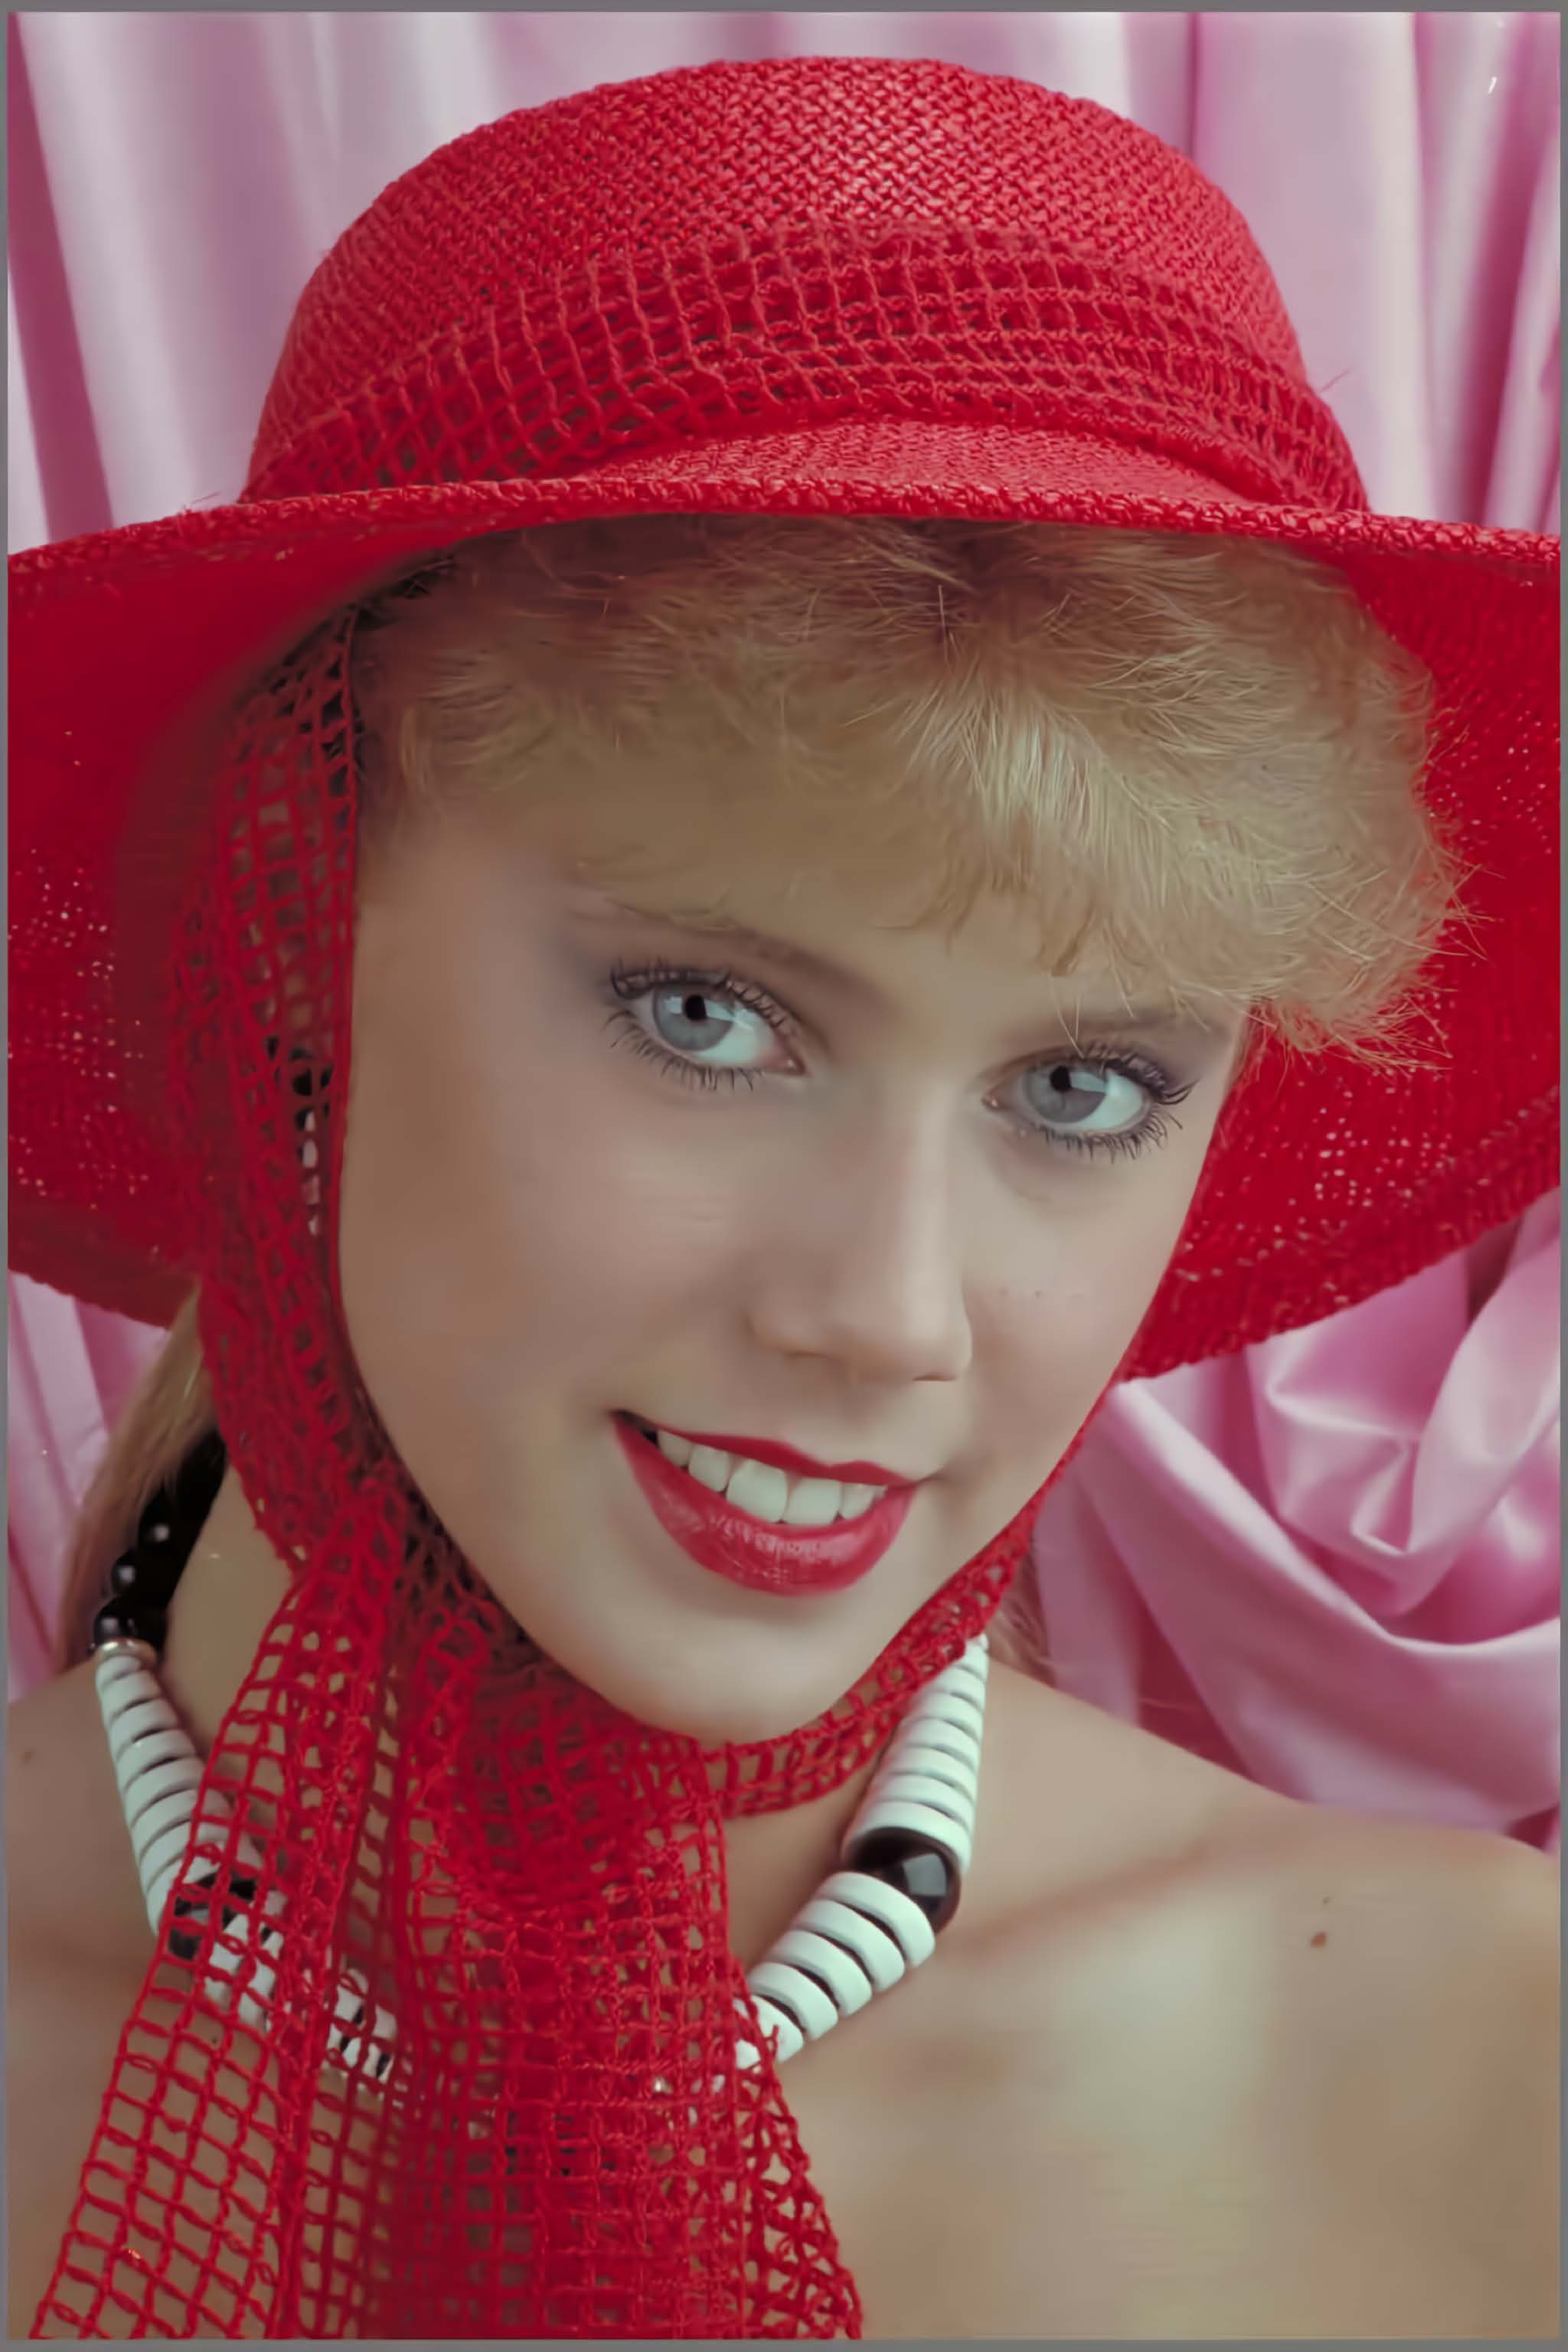
\includegraphics[width=\textwidth]{Immagini/IMAGES/cheng2020_attn_2_IMG0004.pdf}
                \caption{Cheng 0.056bpp}
                \label{fig:ExampleCheng}
            \end{minipage}
            \label{fig:ExamplesCompression}
        \end{figure}
        \footnotetext[1]{\fullcite{KodakDataset}}
    \end{frame}

    % \begin{frame}{Tempi di Compressione}
    %     \begin{figure}[t!]
    %         \centering
    %         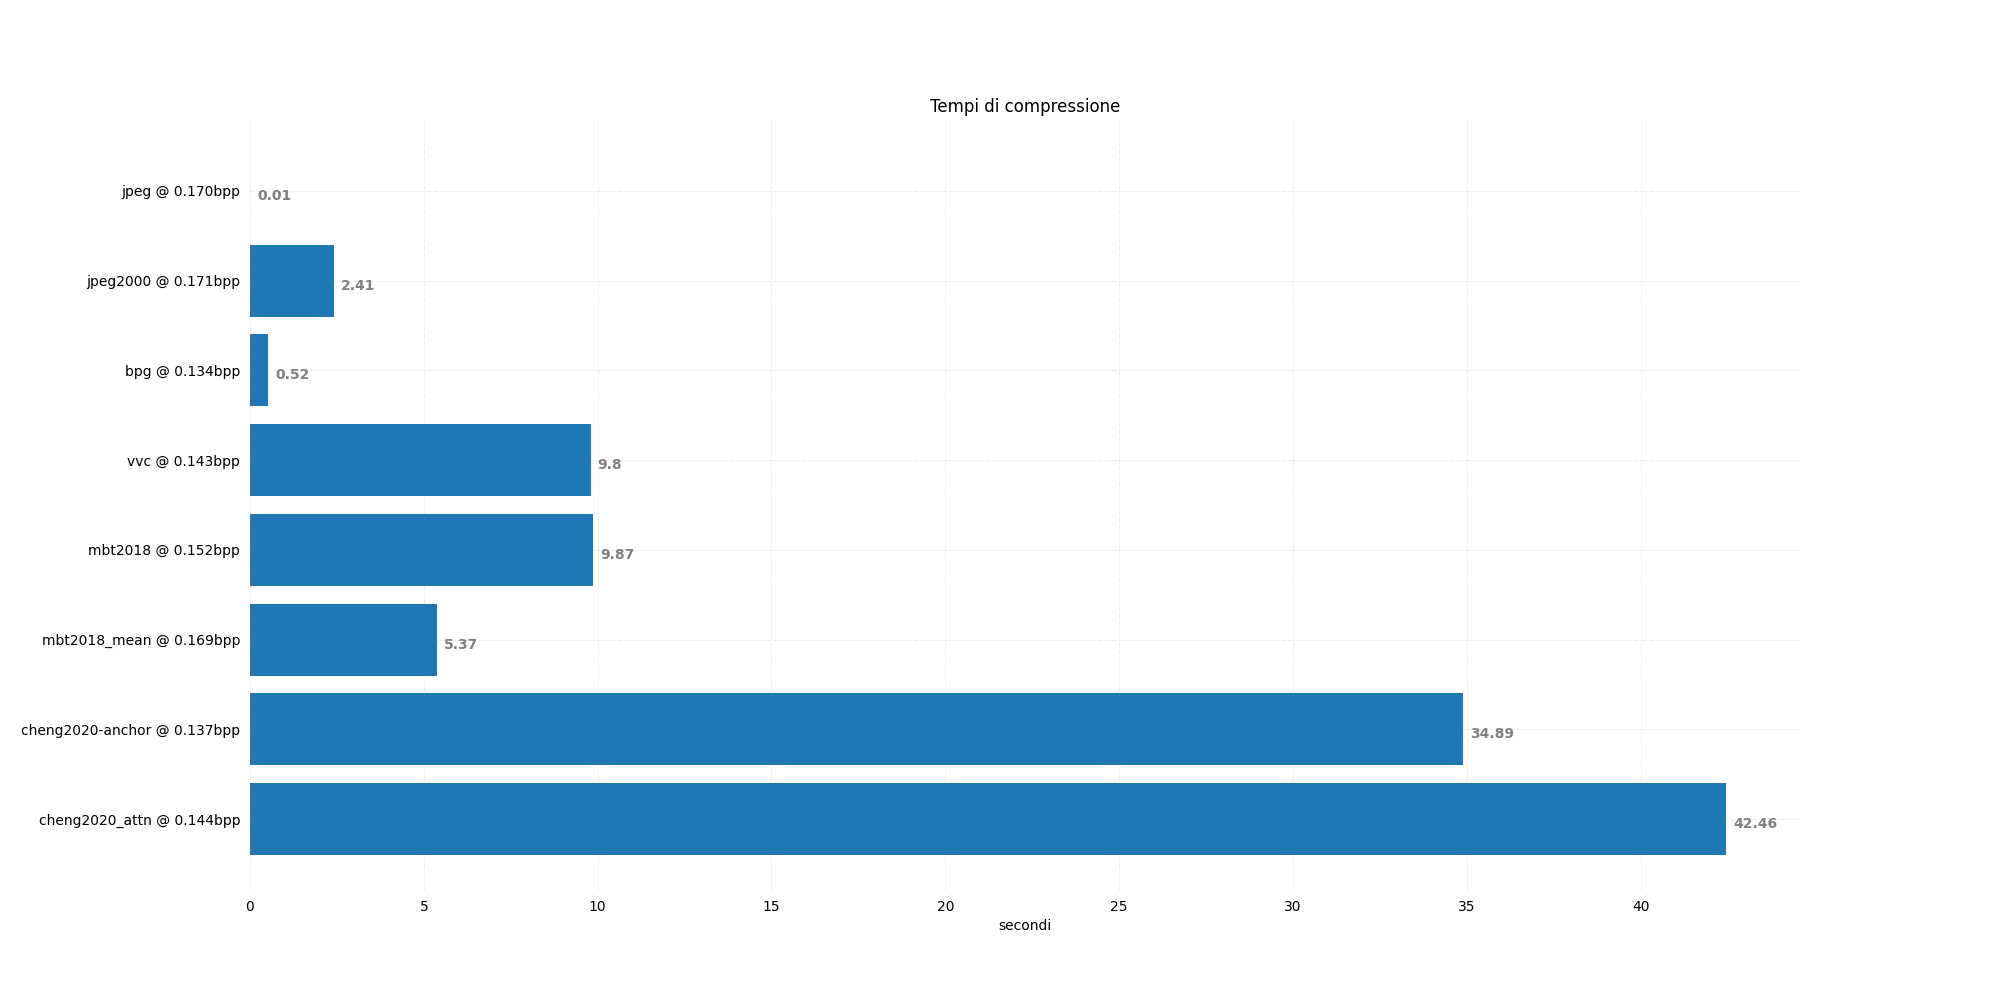
\includegraphics[width=1\textwidth]{Immagini/METRICS/times@0.16bpp.png}
    %         \caption{Tempi di compressione a 0.16 bpp}
    %         \label{fig:times16}
    %     \end{figure}
    % \end{frame}
    \begin{frame}{Tempi di Compressione}
        \begin{figure}[t!]
            \centering
            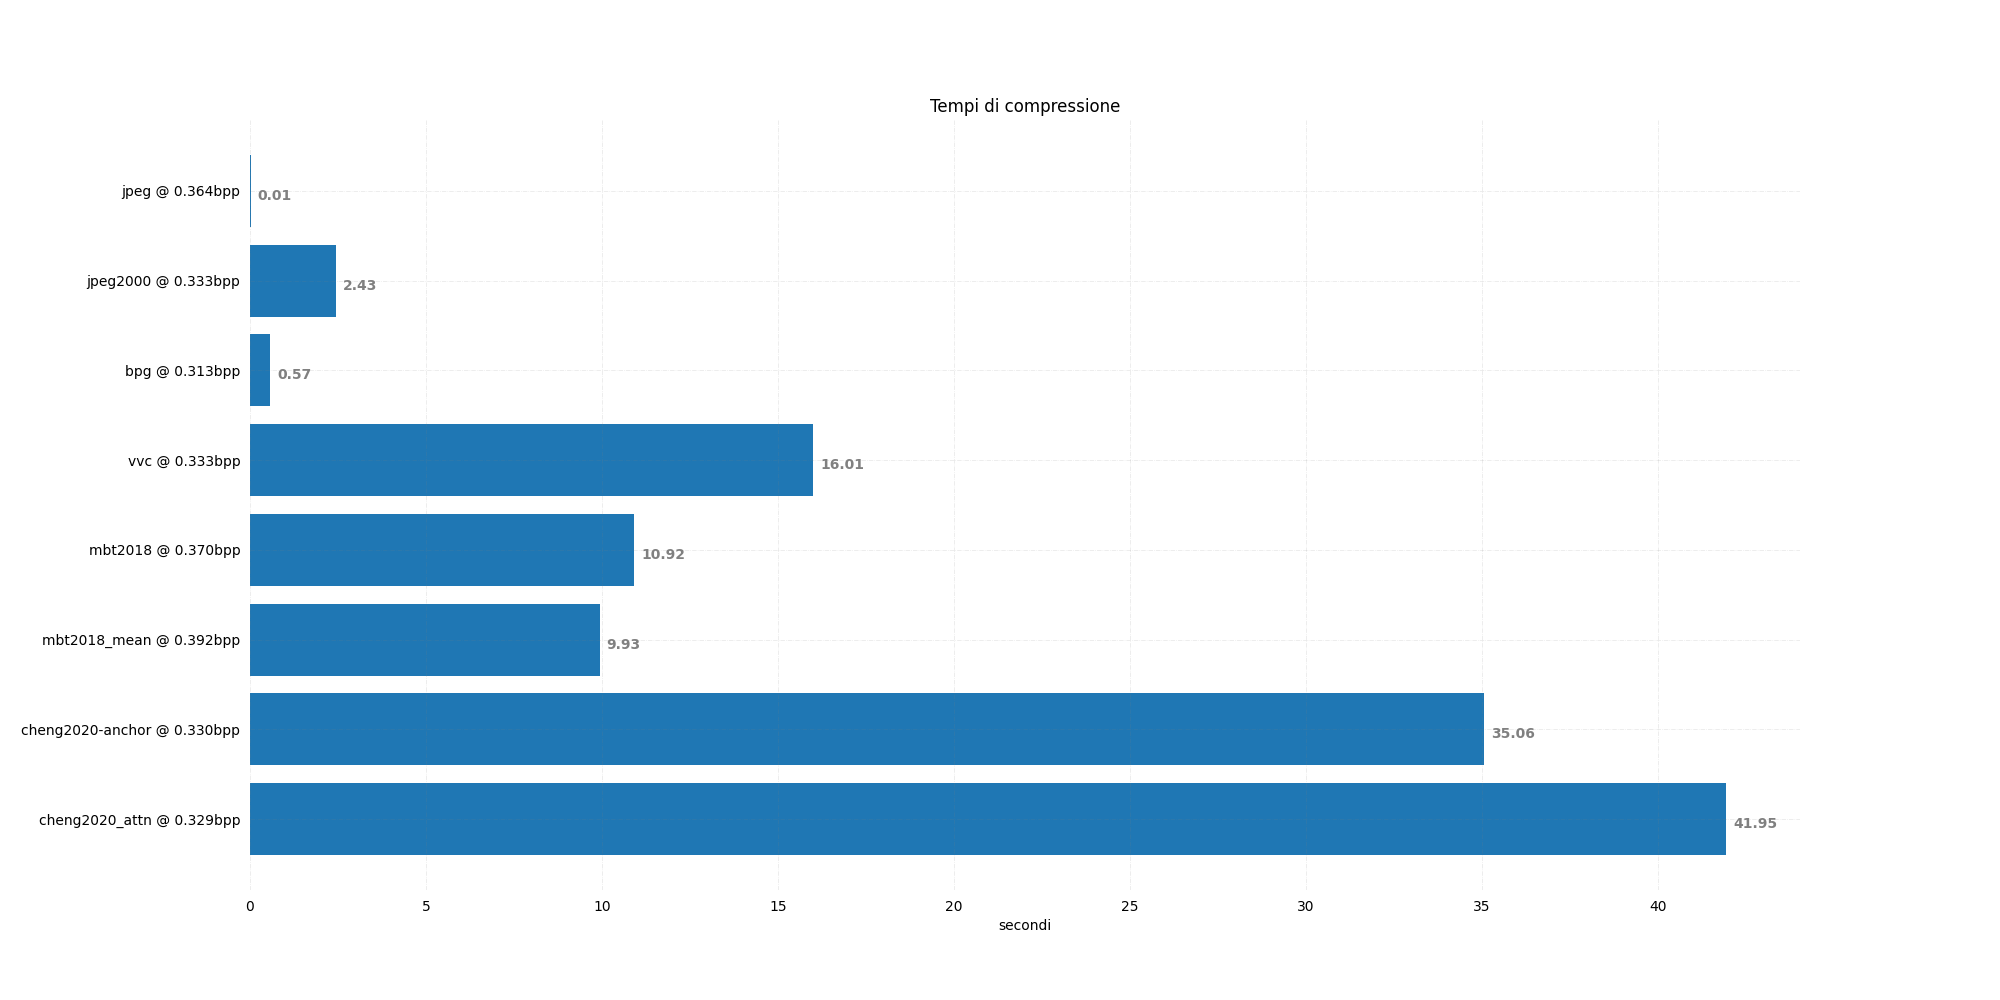
\includegraphics[width=1\textwidth]{Immagini/METRICS/times@0.34bpp.png}
            \caption{Tempi di compressione a 0.34 bpp}
            \label{fig:times34}
        \end{figure}
    \end{frame}

    \begin{frame}{PSNR}
        \begin{figure}[t!]
            \centering
            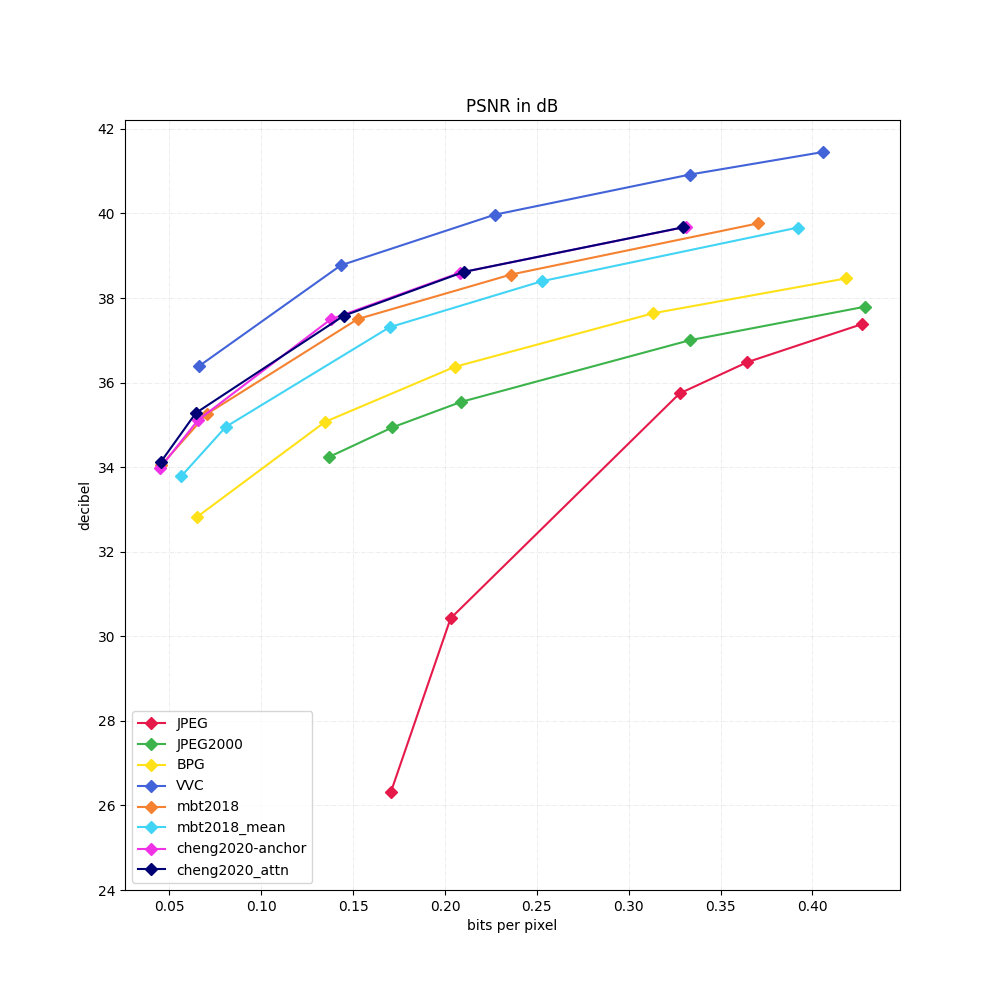
\includegraphics[width=0.57\textheight]{Immagini/METRICS/PSNR.png}
            \caption{Grafico del PSNR, punti corrispondenti alla media delle metriche sulle 24 immagini del dataset}
            \label{fig:GraphPSNR}
        \end{figure}
    \end{frame}

    \begin{frame}{MS-SSIM}
        \begin{figure}[t!]
            \centering
            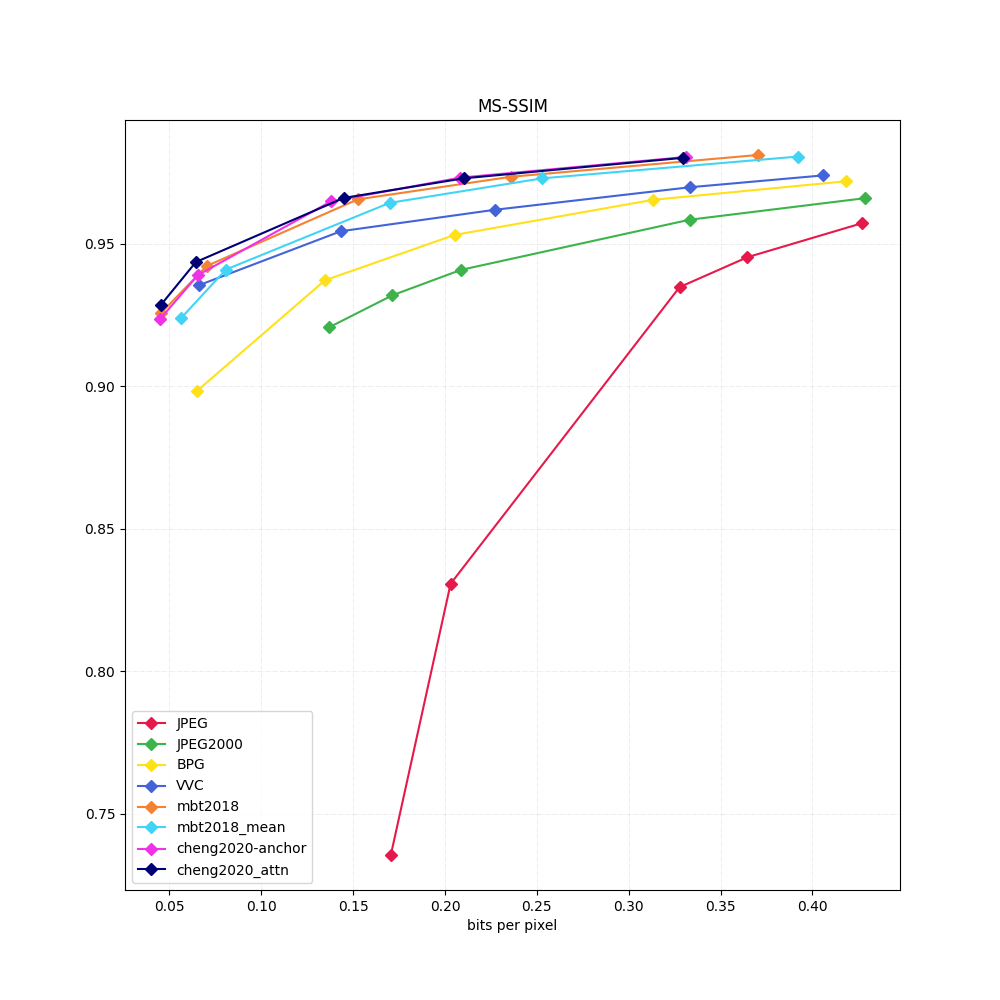
\includegraphics[width=0.57\textheight]{Immagini/METRICS/MS-SSIM.png}
            \caption{Grafico dell'MS-SSIM\footnotemark[1], punti corrispondenti alla media delle metriche sulle 24 immagini del dataset}
            \label{fig:GraphMS-SSIM}
        \end{figure}
        \footnotetext[1]{\fullcite{wang2003multiscale}}
    \end{frame}

    \begin{frame}{LPIPS}
        \begin{figure}[t!]
            \centering
            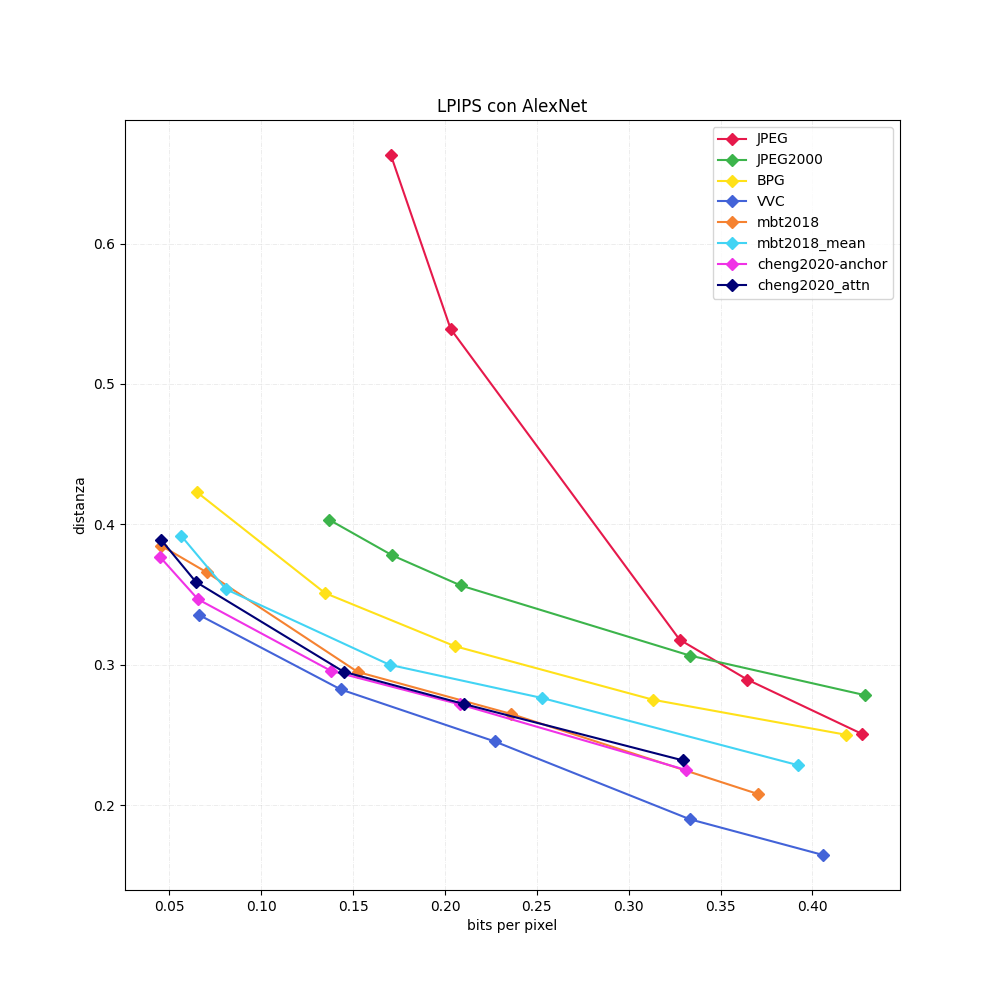
\includegraphics[width=0.57\textheight]{Immagini/METRICS/LPIPS.png}
            \caption{Grafico LPIPS\footnotemark[1] con AlexNet, punti corrispondenti alla media delle metriche sulle 24 immagini del dataset}
            \label{fig:GraphLPIPS}
        \end{figure}
        \footnotetext[1]{\fullcite{zhang2018unreasonable}}
    \end{frame}
    
    
\section{Sviluppi Futuri}

    \begin{frame}{Sviluppi Futuri}
        Durante la ricerca delle informazioni per la stesura di questa tesi ci siamo imbattuti in due lavori molto interessanti
        \begin{itemize}
            \item StructuralADAM \cite{balle2018efficient}
            \item SmallCAE \cite{yang2021slimmable}
        \end{itemize}
    \end{frame}
    

\section{Bibliografia}
    
\begin{frame}[allowframebreaks]{Bibliografia}
    \printbibliography
\end{frame}
    
\begin{frame}{\:}
    \begin{center}
        \large Grazie per la vostra attenzione 
    \end{center}
\end{frame}
    
\end{document}